\documentclass[conference]{IEEEtran}
\IEEEoverridecommandlockouts
% The preceding line is only needed to identify funding in the first footnote. If that is unneeded, please comment it out.
\usepackage{cite}
\usepackage{amsmath,amssymb,amsfonts}
\usepackage{cases}
\usepackage{mathtools}
\usepackage{float}
\usepackage{algorithmic}
\usepackage{graphicx}
\usepackage{textcomp}
\usepackage{xcolor}
\graphicspath{{graphics/}}
\usepackage{longtable}
\usepackage{adjustbox}
\usepackage{scalerel}
\usepackage{tikz}
\usetikzlibrary{svg.path}

\definecolor{orcidlogocol}{HTML}{A6CE39}
\tikzset{
  orcidlogo/.pic={
    \fill[orcidlogocol] svg{M256,128c0,70.7-57.3,128-128,128C57.3,256,0,198.7,0,128C0,57.3,57.3,0,128,0C198.7,0,256,57.3,256,128z};
    \fill[white] svg{M86.3,186.2H70.9V79.1h15.4v48.4V186.2z}
                 svg{M108.9,79.1h41.6c39.6,0,57,28.3,57,53.6c0,27.5-21.5,53.6-56.8,53.6h-41.8V79.1z M124.3,172.4h24.5c34.9,0,42.9-26.5,42.9-39.7c0-21.5-13.7-39.7-43.7-39.7h-23.7V172.4z}
                 svg{M88.7,56.8c0,5.5-4.5,10.1-10.1,10.1c-5.6,0-10.1-4.6-10.1-10.1c0-5.6,4.5-10.1,10.1-10.1C84.2,46.7,88.7,51.3,88.7,56.8z};
  }
}

\newcommand\orcidicon[1]{\href{https://orcid.org/#1}{\mbox{\scalerel*{

\begin{tikzpicture}[yscale=-1,transform shape]
\pic{orcidlogo};
\end{tikzpicture}
}{|}}}}

\usepackage{hyperref}

%\orcidicon{0000-0003-1625-0162}
\hypersetup{draft}
\begin{document}
	
	\title{Comparison of Nature-Inspired and Graph Algorithms Solving Travelling Salesman Problems}
	
	\author{\IEEEauthorblockN{Stefan Eggenschwiler}
		\IEEEauthorblockA{\textit{Institute of Information Systems} \\
			\textit{University of Applied Sciences Northwestern Switzerland}\\
			Olten, Switzerland
			stefan.eggenschwiler@students.fhnw.ch}
		\and
		\IEEEauthorblockN{Maja Spahic-Bogdanovic}
		\IEEEauthorblockA{\textit{Institute of Information Systems} \\
		\textit{University of Applied Sciences Northwestern Switzerland}\\
		Olten, Switzerland
		maja.spahic@students.fhnw.ch}
	}
	
	\maketitle
	
	\begin{abstract}
		This paper is a comparison of two natural-inspired algorithms and five traditional algorithms from graph theory and integer linear programming based on defined key metrics. It focuses on describing the experiment setup, the input models and it outlines the metrics applied in the analysis part. Aim of the analysis is to compare the performance of nature-based algorithms with more conventional algorithms used in the solving of travelling salesman problems (TSP).\\
	\end{abstract}
	
	\begin{IEEEkeywords}
		travelling salesman problem, nature-inspired algorithms, combinatorial optimization
	\end{IEEEkeywords}
	%FINAL PAPER
	\section{Introduction}
 	According to \cite{bernhard2008combinatorial, halim2019combinatorial, gutin2006traveling} a Combinatorial Optimization (CO) problem consists of a limited set of problems with unique components. The goal is to find the optimal combination of each component. The CO problem can be defined by \cite{blum2003metaheuristics}:\newline
 	- a set of variables $X = \{x_1,...,x_n\}$\newline
 	- variable domains $D_1,...,D_n$\newline
 	- constraints among variables\newline
 	- an $objective function$ $f$ to be minimized, where $f:D_1x ... xD_n \xrightarrow{} IR^+$\newline
 	Resulting from this is the set of all possible realizable associations: 
 	$S=\{s=\{(x_1,v_1),...,(x_n,v_n)\} | v_i \in{} D_i, s$ satisfies all the constraints$\}$. According to Blum and Roli \cite{blum2003metaheuristics} $S$ is denoted as a $search \; space$ and all elements of the set can be considered as candidate solutions. For solving a CO problem, it is necessary to find a solution $s^* \in S$ with minimum objective function value, i.e. $f(s^*) \leq f(s) \forall s \in S$. $s^*$ defines the globally optimal solution of $(S,f)$ and $S^* \subseteq S$ the set of globally optimal solutions. Travelling Salesman Problem (TSP) is one the prominent example for CO problems.
	We used twenty-two different TSP problems provided by the University of Heidelberg \cite{tsplib201heidelberg} and TSP algorithm suit (AS) provided by University of Oxford \cite{tsp2019sheridan}. 
	%First we use the existing AS and extend them to be able to run over more than one TSP library. Then we extend the AS with two natural inspired algorithms - Ant-Colony Optimization (ACO) or Particle Swarm Optimization (PSO) and comparing the performance to the greedy..... (algs aufzählen).
	
	\section{Methodology}
	A \textsc{Matlab}\textsuperscript{\textregistered} based TSP algorithm suite developed by the University of Oxford \cite{tsp2019sheridan} served as basis for the experiment setup. The AS was extended by implementing an import functionality allowing the solving of a set of TSP instances published by \cite{tsplib2019} and described in paragraph \ref{problem_set}.\\
 	In a second step, a two nature-inspired algorithms are implemented along the already available algorithms in \cite{tsp2019sheridan}. A list of implemented algorithms is described in the paragraph \ref{algos}.
	\subsection{Optimization Algorithm Selection}\label{algos}
	Several nature-inspired algorithms can be applied to TSP models. According to Abraham et. al \cite{abraham2007swarm} Ant-Colony Optimization (ACO) and Particle Swarm Optimization (PSO) are two most popular algorithm in the field of swarm intelligence. On that account, we choose this two algorithm. 

	\subsection{Problem Set}\label{problem_set}
	The set of TSP instances used in the experiment consists of twenty-two problems varying in size and complexity. The problems were published by \cite{tsplib2019} and are considered as standard in this field of research. TSP problem instances vary from a size between 14 and 2392 nodes. In addition, an optimal solution exists for each instance. This optimal solution is important to compute the accuracy of an algorithm.
	
	\subsection{Metric Definition}\label{metric}
	In order to be able to compare the performance of different algorithms, meaningful metrics have been defined. In the implemented solution, successfully solving a TSP instance yields two values:
	\begin{itemize}
		\item Execution time
		\item Edge distance of the solution
	\end{itemize}
	The execution time is a non-deterministic metric due to its platform dependency and various potential side effects during the execution (other running processes on the platform), whereas the edge distance of different algorithms or executions can be directly compared to each other.
	
	\section{Optimization Problem}
	\subsection{Traveling Salesman Problem}
	The TSP investigates the question, which route the salesman should take in order to travel from one city to the next with minimum distance cost and without visiting a city more than once \cite{bernhard2008combinatorial, tsp2019sheridan, moustapha2016advances}. The TSP can be modelled as undirected graph\footnote{formed through symmetric TSP, where the distance between two cities is the same in any opposite direction} or as a complete graph\footnote{formed through asymmetric TSP, where the path may not exist or the distance in both direction can be different} \cite{gutin2006traveling}. 
	Traditionally, TSP can be defined as an integer linear programming (ILP) model. Three of the most common formulations of TSP are Dantzig-Fulkerson-Johnson (DFJ), Miller-Tucker-Zemlin (MTZ) and Sarin–Sherali–Bhootra (SSB) \cite{moustapha2016advances, gutin2006traveling}. 
	In order to calculate the optimal route, e.g. brute force searching method can be used. Hereby, all possible permutations will be formed to find the most favorable one route. Likewise, heuristic methods can be used to find the optimal route, such as nearest neighbours\cite{halim2019combinatorial}. 

	\subsection{TSPlib}
	For our analysis, we rely a widely used library of tsp instances TSPLIB 95\cite{tsplib2019}. The library contains instances of various size and node count, therefore being ideal for performing a benchmark analysis. Additionally, all instances are provided with an optimal distance. It is therefore possible to calculate the overall accuracy of an algorithm and compare it to others.
	
	\section{Optimization Algorithm}
	Table \ref{tab:classification} show used algorithm, there shortcuts and the naming used in the analysis:
		\begin{table}[h]
	    \centering
	    \begin{tabular}{ | l | l | l | }
	         \hline
        	Shortcut & Algorithm & Name in the Analysis \\ \hline \hline
        	ACO & Ant-Colony Optimization & aco-50\\
        	    &                         & aco-100\\ \hline
        	SPSO & Standard & pso-qpso-50\\
                &  Particle Swarm Optimization & pso-spso-100\\
                &                         & pso-spso-150\\
                &                         & pso-spso-200\\ \hline
        	APSO & Adaptive & pso-apso-50\\
                &  Particle Swarm Optimization & pso-apso-100\\
                &                         & pso-apso-150\\
                &                         & pso-apso-200\\ \hline
            QPSO & Quantum-behaved & pso-qpso-50\\
                &  Particle Swarm Optimization & pso-qpso-100\\
                &                         & pso-qpso-150\\
                &                         & pso-qpso-200\\ \hline
                & Increasing loop algorithm & inc\_loop \\ \hline
                & Forcefully increasing loop algorithm & f\_inc\_loop \\ \hline
                & Optimal greedy algorithm & opt\_greedy \\ \hline
                & 2-opt algorithm & two\_opt \\ \hline
	    \end{tabular}
	    \caption{List of used Algorithms and there shorts cuts}
	    \label{tab:classification}
	\end{table}
	
	
	\subsection{Ant Colony Optimization}
	In his Ph.D Thesis, Marco Dorigo introduced in 1992 the Ant Colony Optimization (ACO) algorithm \cite{halim2019combinatorial, abraham2007swarm}. ACO is a probabilistic approach to solve computational problems which can be reduced to finding good paths through graphs \cite{abraham2007swarm}. 
	
	According to Halimi et al. \cite{halim2019combinatorial} inspiration for this algorithm comes from the observation of ants colony searching for food. Ants foraging for food are distributed in different directions \cite{messac2015optimization}. 
	Adapted to the TSP, the artificial ant is an agent that moves from one city to the next \cite{halim2019combinatorial}. In the search for food, ants leave a substance called pheromone along the path, which in turn helps to identify the route later again. The choice of the city to travel is based on the probabilistic function and within this probability the artificial ant selects the new cities by edges, accumulation of pheromone traces and proximity to the ant. On the ACO algorithm, three ideas of ant behavior are transferred: (1) choice of path is based on a high pheromone value, (2) a higher pheromone concentration along shorter paths, and (3) use of the path for communication purposes between the ants \cite{halim2019combinatorial}. 
	
	
% 	Probability to choose city $s$ of an ant $k$ in city $r$, which is not belong to working memory $M_k$ as in \ref{eq:aco1}:
% \begin{equation}\label{eq:aco1}
% \end{equation}
%  $
%  	   s=\begin{CASES}  
% arg_{u \neq M_{k}}max\left\{   \left[\tau\left(r,u\right)\right]* \left[\eta\left(r,u\right)\right] ^{\beta}
%                      \right\} \;if \;q < q_{0}  \\
% S\;\;\;\;\;\;\;\;\;\;\;\;\;\;\;\;\;\;\;\;\;\;\;\;\;\;\;\;\;\;\;\;\;\;\;\;\;\;\;\;\;\;\;\;\;\;\;\;\;\;\;\;\; \;\;\;\;\;\;\;otherwise
% \end{CASES}
% $\newline


% $\tau\left(r,u\right)$ describes amount of the pheromone trail on edge $\left(r,u\right)*\eta\left(r,u\right)$. This is the heuristic function describing the inverse of the distance between cities $r$ and $u$. $\beta$ represent the weightage of the pheromone trail and closeness, $q$ represent a random value delivered from uniform distribution $[0,1]$ and $q_0:(0\leq q_0\leq1)$ represent the threshold parameter. $S$ represent a random variable, which is selected based o the probability distribution, offering edges 

	\subsection{Particle Swarm Optimization}
    The Particle Swarm Optimization (PSO) was inspired by birds seeking for food and imitates their swarm behavior \cite{abraham2007swarm, messac2015optimization}. PSO search algorithm is initiated with a set of random solutions called particles. Inspired by the behavior of a swarm of birds - synchronized movements, they move without collision and they maintain distance between them-, the population seeks the global optimum. The motion of each particle is governed by a velocity update equation. This strategy involves each individual remembering or recording the places of the best fitness. An individual's best solution or success is called the best particle, and this information is then shared with neighbors. Usually, a swarm is designed by particles in a multidimensional space, and each particle in each iteration has a position and velocity \cite{abraham2007swarm, messac2015optimization}. Besides the standard implementation for the PSO algorithm, we consider two extended version of the algorithm in our analysis. In the following chapters, both of them will be introduced.

	\subsubsection{Adaptive Particle Swarm Optimization}
	The Adaptive Particle Swarm Optimization algorithm (APSO) is based on the original PSO algorithm. According to \cite{apso2009}, it distinguishes itself through three modifications:
	\begin{enumerate}
        \item The search space is divided into multiple segments, like a spider net. Each segment is populated individually, therefore highly increasing the search accuracy of the algorithm.
        \item Each sub-swarm shares information with its neighbours. Swarms with higher fitness values will therefore guide their colleges, hence improving their fitness as well. This idea is taken from the flocking behaviour of spiders.
        \item APSO uses the fitness value to adjust the learning factors ($c1, c2$). In the standard PSO, the fitness is not taken in consideration.
    \end{enumerate}
	\subsubsection{Quantum-behaved Particle Swarm Optimization}
	The Quantum-behaved Particle Swarm Optimization algorithm (QPSO) is based on the principles of quantum mechanics \cite{Yumin2014} and was first introduced by \cite{Sun2004ParticleSO}. It outperforms the standard implementation of the PSO algorithm, but has less customizable parameters. The computation of the algorithm can be depicted in the flowchart in Figure \ref{fig:qpso}.
	\begin{enumerate}
        \item First the parameters will be initialized
        \item Then, the individual fitness values are computed
        \item The optimal population history is updated. If a particle has a better fitness than the population's optimum, the optimum is updated.
        \item The overall optimum of particles is updated. If the fitness of a particle is lower than the global optimum, it will be replaced by it.
        \item Updates all particles by using the quantum-behaved algorithm formula.
        \item The algorithm repeats steps two to five until it reaches the maximum number of iterations and terminates.
    \end{enumerate}
	
	\begin{figure}[h]
    		\centering
    		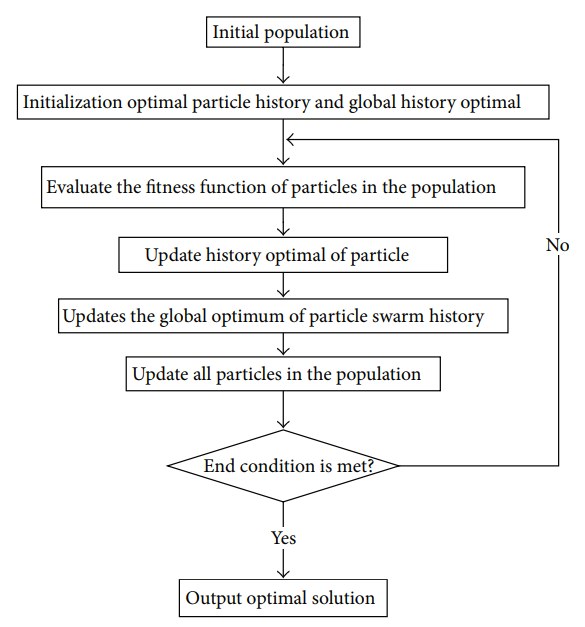
\includegraphics[width=\textwidth/2]{qpso.PNG}
    		\caption{QPSO algorithm flowchart\cite{Yumin2014}}
    		\label{fig:qpso}
	\end{figure}
	
	\subsection{Increasing loop algorithm}\label{inc_loop}
	Increasing loop is a stochastic algorithm producing a possible solution, which has a high possibility to be optimal. At the beginning, the algorithm randomly selects three vertices and forms a loop with them. It then randomly adds another adjusted vertex to the sub-loop and calculate the new distance. The algorithm then calculates if there could be built a shorter loop. It evaluates the added distance from replacing each existing connection. It remembers the increased distance and repeats this for all nodes not in the sub-loop, therefore finding what the global minimal deformation for the sub-loop would be if it included one of the unconnected nodes. The algorithm then forms this new minimal connection, and then recomputes the minimal global deformation. This process will be executed iteratively until it runs out of unconnected vertices. This procedure is visualized in Figure \ref{fig:increasing_loop}.
	
	\begin{figure}[h]
    		\centering
    		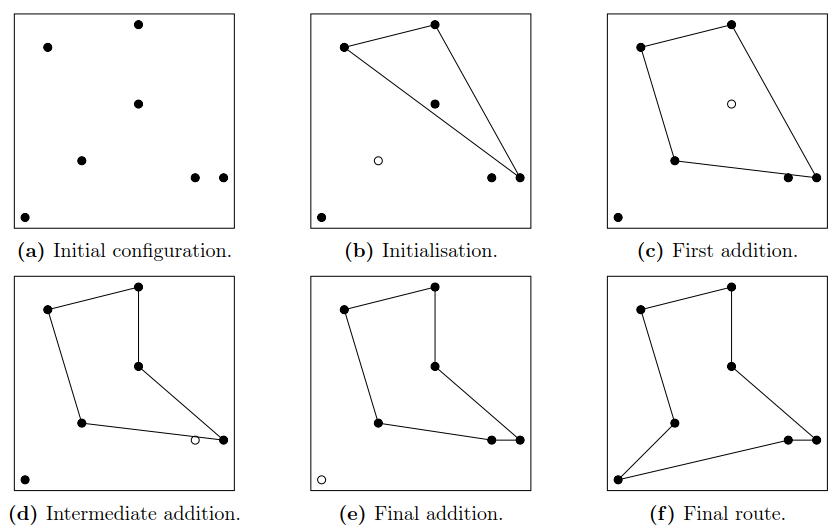
\includegraphics[width=\textwidth/2]{increasing_loop.PNG}
    		\caption{Increasing loop algorithm \cite{tspalgo2016}}
    		\label{fig:increasing_loop}
	\end{figure}
	    
	\subsection{Forcefully increasing loop algorithm}
	The forcefully increasing loop algorithm is a faster implementation of the increasing loop algorithm \ref{inc_loop}. At the beginning, it randomly selects three vertices and forms a loop with them. It then randomly adds another adjusted vertex to the sub-loop and calculate the new distance. The algorithm then calculates if there could be built a shorter loop.
	\subsection{Optimal greedy algorithm}
	The Optimal greedy algorithm is a subset of the greedy algorithm which follows the heuristic of choosing a locally optimal solution at each step in order to find the global optimum \cite{greedy2005}. It does usually not produce an optimal solution, but it is a reasonable trade-off between computation time and optimality. The Optimal greedy algorithm differs from this by using specific starting nodes. It compares the edge cost of all computed routes and chooses the path with the minimal distance.
	\subsection{2-opt algorithm}
	2-opt is an iterative algorithm \cite{2opt1958} optimizing Hamiltonian cycles by randomly removing two edges and then altering the cycle by cross-linking the four nodes with one another as depicted in Figure \ref{fig:2opt}. Afterwards, the distance of the cycle is calculated and compared to the previously best distance and takes whichever is lower. For this analysis, the algorithm terminates if it does not improve its best solution over 1000 consecutive iterations.
	
	\begin{figure}[h]
    		\centering
    		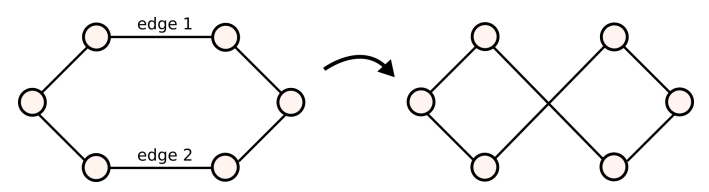
\includegraphics[width=\textwidth/2]{twoopt.PNG}
    		\caption{Hamiltonian cycle optimization \cite{tspalgo2016}}
    		\label{fig:2opt}
	\end{figure}
	
	\section{Performance Comparison of selected Optimization Algorithm}
	This chapter discuss the output of the simulations using \textsc{Matlab}\textsuperscript{\textregistered}. The output was analyzed according to the execution time and the distance compered to optimal distance. The execution time is the duration in seconds consumed to solve a specific TSP problem. For the nature-inspired algorithms ACO and PSO, different amount of population (50, 100, 150 and 200) was defined. Because of time consuming purpose the ACO algorithm was running only with a population of 50 and 100 ants; the simulation with 150 or 200 ants would need to run few days to solve the chosen TSP problems. Table \ref{tab:parameter} provides information about the specified parameters.
	\begin{table}[H]
    	\centering
    	\begin{tabular}{l | l l l}
    		Algo. & Parameters \\
    		\hline
    		ACO   & \begin{tabular}[c]{@{}l@{}}Iteration = 200\\ Num of Ants = 50, 100\\ $\alpha$ (pheromone exponent) = 1\\ $\beta$ (desirability exponent) = 1\\ $\rho$ (evaporation rate) = 0.5\end{tabular} \\
    		\hline
    		APSO  & \begin{tabular}[c]{@{}l@{}}Iteration = 400\\ Population Size = 50, 100, 150, 200\\ $\alpha$ = 0.8\\ $\beta$ = 0.9\\ $\gamma$ = 0.99\end{tabular}                                                      \\
    		\hline
    		QPSO  & \begin{tabular}[c]{@{}l@{}}Iteration = 400\\ Population Size = 50, 100, 150, 200\\ $\alpha$ min. = 0.08\\ $\alpha$ max. = 0.9\end{tabular}                                                      \\
    		\hline
    		SPSO  & \begin{tabular}[c]{@{}l@{}}Iteration = 400\\ Population Size = 50, 100, 150, 200\\ c1,c2 (learning factors) = 1.0\\ w (momentum of inertia) = 0.9\end{tabular}
    	\end{tabular}
    	\caption{Parameter settings for nature algorithms}
    	\label{tab:parameter}
    \end{table} 

	In the simulation each algorithm was running 100 times with twenty-two benchmark problems from TSPlib \cite{tsplib2019}. Table \ref{tab:tspgroupbynodesize} shows the proposed TSP problems with the optimum distance. The TSP problems were added to a range according to the node size: "Small" $(n<100)$, "Medium" $(99<n<200)$ and "Big" $(n>199)$. The partitioning was made by taking into account the number of nodes and the time needed to solve the TSP problem. 
	\begin{table}[H]
	    \centering
	    \begin{tabular}{ | l | l | l | l | }
	         \hline
        	TSP & Optimal Distance & Nodes & Classification \\ \hline \hline
        	berlin52 & 7542 & 52 & Small \\ \hline
        	burma14 & 3323 & 14 & Small \\ \hline
        	eil51 & 426 & 51 & Small \\ \hline
        	eil76 & 538 & 76 & Small \\ \hline
        	gr96 & 55209 & 96 & Small \\ \hline
        	pr76 & 108159 & 76 & Small \\ \hline
        	st70 & 675 & 70 & Small \\ \hline
        	ulysses16 & 6859 & 16 & Small \\ \hline
        	ulysses22 & 7013 & 22 & Small \\ \hline
        	ch130 & 6110 & 130 & Medium \\ \hline
        	ch150 & 6528 & 150 & Medium \\ \hline
        	eil101 & 629 & 101 & Medium \\ \hline
        	kroA100 & 21282 & 100 & Medium \\ \hline
        	kroC100 & 20749 & 100 & Medium \\ \hline
        	kroD100 & 21294 & 100 & Medium \\ \hline
        	lin105 & 14379 & 105 & Medium \\ \hline
        	rd100 & 7910 & 100 & Medium \\ \hline
        	gr202 & 40160 & 202 & Big \\ \hline
        	gr666 & 294358 & 666 & Big \\ \hline
        	pr1002 & 259045 & 1002 & Big \\ \hline
        	pr2392 & 378032 & 2392 & Big \\ \hline
        	tsp225 & 3916 & 225 & Big \\ \hline
	    \end{tabular}
	    \caption{Classification of TSP based on node size}
	    \label{tab:tspgroupbynodesize}
	\end{table}








    \subsection{Execution Time}
	    
	  \begin{figure}[h]
    		\centering
    		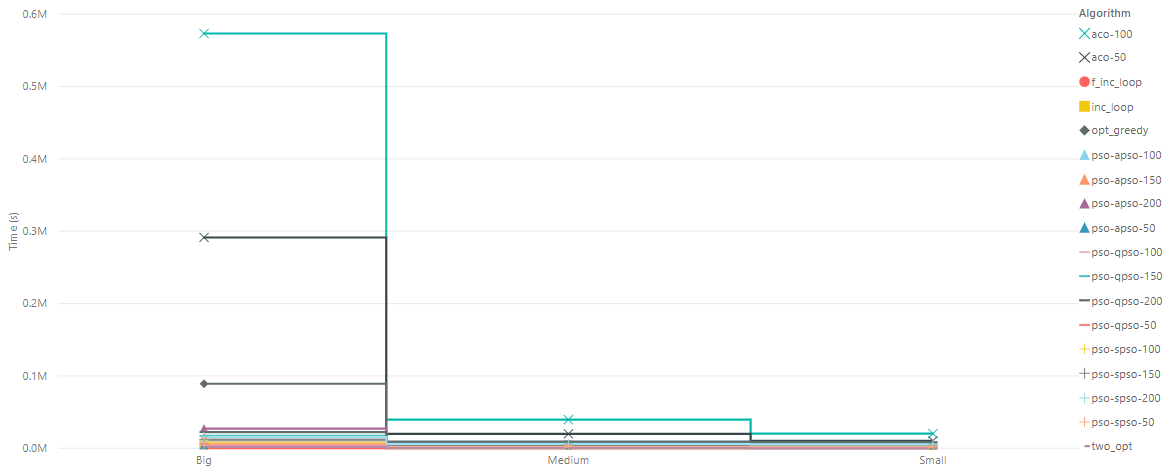
\includegraphics[width=\columnwidth]{time_goupNodeSize.png}
    		\caption{Comparison time to node size}
    		\label{fig:boxPlotTime}
	    \end{figure}
	   
	  \begin{figure}[h]
    		\centering
    		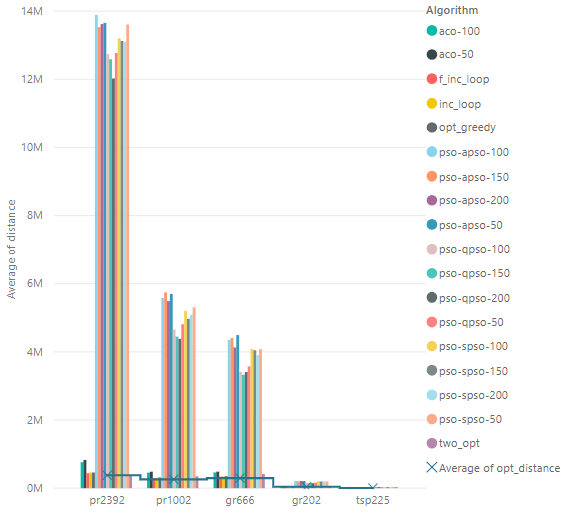
\includegraphics[width=\columnwidth]{distance_opt_dostance_big.png}
    		\caption{Average distance compared to optimal distance for Big}
    		\label{fig:distanceBig}
	    \end{figure}
	    
	      \begin{figure}[h]
    		\centering
    		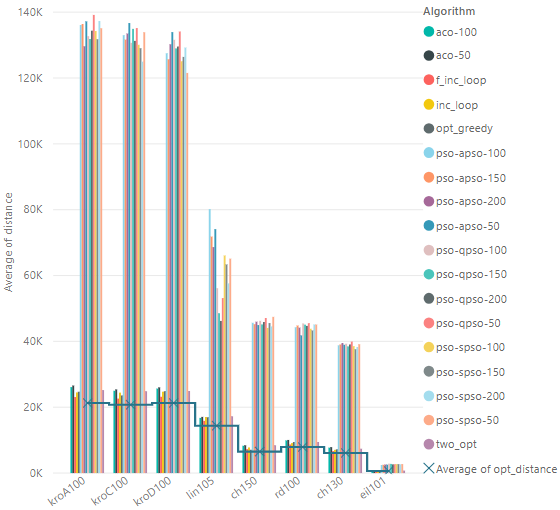
\includegraphics[width=\columnwidth]{distance_opt_dostance_medium.png}
    		\caption{Average distance compared to optimal distance for Medium}
    		\label{fig:distanceMedium}
	    \end{figure}
	    
	    \begin{figure}[h]
    		\centering
    		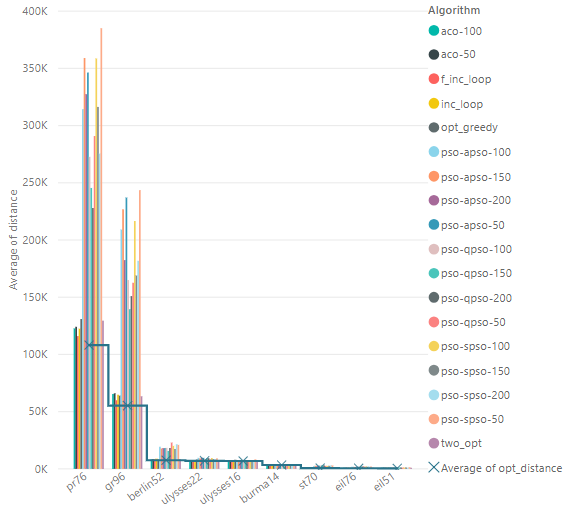
\includegraphics[width=\columnwidth]{distance_opt_dostance_small.png}
    		\caption{Average distance compared to optimal distance for Small}
    		\label{fig:distanceSmall}
	    \end{figure}
	 
    \subsection{Edge Distance of the Solution}
    
    \begin{table}[h]
	    \centering
	    \begin{adjustbox}{width=\columnwidth}
	    \begin{tabular}{ | l | l | l | l | l | l | l | l | l | l | }
	         \hline
   TSP & aco-100 & aco-50 & f\_inc\_loop & inc\_loop & opt\_greedy & pso-apso-100 & pso-apso-150 & pso-apso-200 & pso-apso-50  \\ \hline\hline
berlin52 & 9.21 \% & 10.58 \% & 11.71 \% & 16.91 \% & 8.49 \% & 155.87 \% & 135.43 \% & 139.96 \% & 139.4 \%  \\ \hline
burma14 & 0.05 \% & 0.19 \% & 3.13 \% & 3.43 \% & 15.59 \% & 9.75 \% & 13.63 \% & 15.53 \% & 7.88 \%  \\ \hline
ch130 & 25.97 \% & 28.87 \% & 9.17 \% & 15.49 \% & 17.82 \% & 534.96 \% & 539.04 \% & 546.56 \% & 537.62 \%  \\ \hline
ch150 & 26.77 \% & 29.17 \% & 11.28 \% & 18.99 \% & 8.43 \% & 599.05 \% & 592.51 \% & 604.11 \% & 588.65 \%  \\ \hline
eil101 & 27.62 \% & 29.37 \% & 11.08 \% & 14.18 \% & 17.07 \% & 287.75 \% & 298.16 \% & 307.47 \% & 303.69 \%   \\ \hline
eil51 & 13.6 \% & 15.73 \% & 8.15 \% & 13.21 \% & 18.73 \% & 128.5 \% & 125.31 \% & 121.95 \% & 165.03 \%   \\ \hline
eil76 & 18.6 \% & 20.4 \% & 10.07 \% & 12.47 \% & 13.88 \% & 235.87 \% & 212 \% & 218.85 \% & 246.27 \%   \\ \hline
gr202 & 31.49 \% & 34.46 \% & 9.36 \% & 15.97 \% & 17.18 \% & 425.93 \% & 392.54 \% & 427.59 \% & 415.26 \%   \\ \hline
gr666 & 55.83 \% & 63.66 \% & 13.67 \% & 17.91 \% & 18.99 \% & 1378.37 \% & 1396.86 \% & 1302.61 \% & 1425.98 \%   \\ \hline
gr96 & 18.22 \% & 19.55 \% & 8.56 \% & 17.29 \% & 15.82 \% & 278.72 \% & 310.73 \% & 230.43 \% & 329.35 \%   \\ \hline
kroA100 & 22.64 \% & 24.88 \% & 8.5 \% & 15.07 \% & 16.05 \% & 539.49 \% & 540.91 \% & 509.1 \% & 544.63 \%   \\ \hline
kroC100 & 20.41 \% & 22.43 \% & 8.97 \% & 17.71 \% & 13.58 \% & 541 \% & 534.47 \% & 543.35 \% & 558.78 \%   \\ \hline
kroD100 & 20.41 \% & 22.2 \% & 8.83 \% & 16.04 \% & 16.73 \% & 498.77 \% & 490.18 \% & 511.62 \% & 528.97 \%   \\ \hline
lin105 & 16.49 \% & 18.65 \% & 10.3 \% & 18.39 \% & 17.81 \% & 457.53 \% & 399.37 \% & 377.33 \% & 415.26 \%   \\ \hline
pr1002 & 75.19 \% & 86.16 \% & 12.77 \% & 16.28 \% & 20.53 \% & 2056.53 \% & 2118.24 \% & 2019.16 \% & 2100.62 \%   \\ \hline
pr2392 & 100.72 \% & 119.04 \% & 15.76 \% & 20.62 \% & 21.36 \% & 3573.67 \% & 3478.95 \% & 3503.32 \% & 3512.35 \%   \\ \hline
pr76 & 13.46 \% & 14.79 \% & 7.27 \% & 13.2 \% & 21.04 \% & 190.59 \% & 231.95 \% & 202.72 \% & 220.18 \%   \\ \hline
rd100 & 25.05 \% & 27.15 \% & 9.71 \% & 14.88 \% & 19.18 \% & 459.74 \% & 466.3 \% & 458.18 \% & 428.55 \%   \\ \hline
st70 & 18.09 \% & 19.83 \% & 7.34 \% & 11.88 \% & 12.84 \% & 267.49 \% & 292.4 \% & 267.04 \% & 311.54 \%   \\ \hline
tsp225 & 40.86 \% & 45.71 \% & 10.29 \% & 14.02 \% & 18.31 \% & 725.32 \% & 729.33 \% & 732.37 \% & 749.43 \%   \\ \hline
ulysses16 & 0.02 \% & 0.17 \% & 3.25 \% & 6.73 \% & 15.8 \% & 7.28 \% & 1.36 \% & 8.3 \% & 7.61 \%   \\ \hline
ulysses22 & 0.76 \% & 1.08 \% & 4.27 \% & 8.56 \% & 16.64 \% & 36.87 \% & 29.39 \% & 36.96 \% & 36.6 \%   \\ \hline
	    \end{tabular}
	    \end{adjustbox}
	    \caption{Deviation of distance to optimal distance - Part I}
	    \label{tab:deviationp1}
	\end{table}
	
    \begin{table}[h]
	    \centering
	    \begin{adjustbox}{width=\columnwidth}
	    \begin{tabular}{ | l | l | l | l | l | l | l | l | l | l | }
	         \hline
   TSP & pso-qpso-100 & pso-qpso-150 & pso-qpso-200 & pso-qpso-50 & pso-spso-100 & pso-spso-150 & pso-spso-200 & pso-spso-50 & two\_opt \\ \hline
berlin52 & 142.74 \% & 107.47 \% & 141.08 \% & 203.87 \% & 166.27 \% & 130.15 \% & 185.08 \% & 177.45 \% & 10.74 \% \\ \hline
burma14 & 11.13 \% & 2.14 \% & 1.38 \% & 3.7 \% & 2.02 \% & 5.54 \% & 15.44 \% & 17.12 \% & 2.23 \% \\ \hline
ch130 & 542.74 \% & 529.64 \% & 539.24 \% & 553.38 \% & 530.77 \% & 515.55 \% & 526.72 \% & 540.34 \% & 20.92 \% \\ \hline
ch150 & 608.32 \% & 591.45 \% & 602.75 \% & 621.46 \% & 575.3 \% & 597.92 \% & 582.28 \% & 626.78 \% & 29.31 \% \\ \hline
eil101 & 351.51 \% & 341.02 \% & 318.54 \% & 324.41 \% & 328.65 \% & 329.67 \% & 321.56 \% & 333.73 \% & 17.89 \% \\ \hline
eil51 & 144.51 \% & 180.54 \% & 169.21 \% & 154.39 \% & 156.37 \% & 177.71 \% & 142.68 \% & 230.62 \% & 9.07 \% \\ \hline
eil76 & 266.02 \% & 266.09 \% & 274.91 \% & 269.84 \% & 270.91 \% & 238.79 \% & 262.01 \% & 274.64 \% & 14.24 \% \\ \hline
gr202 & 269.39 \% & 260.22 \% & 258.15 \% & 301.92 \% & 400.36 \% & 382.3 \% & 380.11 \% & 383.67 \% & 22.09 \% \\ \hline
gr666 & 1058.03 \% & 1030.08 \% & 1057.8 \% & 1114.13 \% & 1287.76 \% & 1274.82 \% & 1225.52 \% & 1285.74 \% & 42.42 \% \\ \hline
gr96 & 198.77 \% & 152.71 \% & 173.46 \% & 194.53 \% & 292.31 \% & 205.94 \% & 229.31 \% & 341.14 \% & 14.83 \% \\ \hline
kroA100 & 523.55 \% & 519.44 \% & 531.37 \% & 553.89 \% & 530.88 \% & 519.21 \% & 545.19 \% & 534.85 \% & 18.41 \% \\ \hline
kroC100 & 529.78 \% & 550.26 \% & 532.65 \% & 551.43 \% & 526.93 \% & 521.91 \% & 502.21 \% & 545.29 \% & 19.76 \% \\ \hline
kroD100 & 518 \% & 505.71 \% & 508.41 \% & 529.77 \% & 487.37 \% & 493.61 \% & 506.85 \% & 470.75 \% & 17.05 \% \\ \hline
lin105 & 290.5 \% & 237.59 \% & 221.36 \% & 269.62 \% & 359.49 \% & 340.52 \% & 300.7 \% & 352.87 \% & 19.9 \% \\ \hline
pr1002 & 1696.65 \% & 1615.92 \% & 1591.54 \% & 1756.37 \% & 1909.26 \% & 1818.39 \% & 1864.57 \% & 1947.8 \% & 34.43 \% \\ \hline
pr2392 & 3270.02 \% & 3229.1 \% & 3080.47 \% & 3277.79 \% & 3392.83 \% & 3372.39 \% & 3365.01 \% & 3499.16 \% & 0.01 \% \\ \hline
pr76 & 152.07 \% & 126.97 \% & 110.76 \% & 168.91 \% & 231.57 \% & 192.43 \% & 154.7 \% & 256.06 \% & 19.71 \% \\ \hline
rd100 & 474.41 \% & 469.83 \% & 465.09 \% & 475.46 \% & 454.04 \% & 447.49 \% & 470.2 \% & 470.17 \% & 19.35 \% \\ \hline
st70 & 326.56 \% & 326.66 \% & 331.2 \% & 286.17 \% & 283.47 \% & 290.31 \% & 330.54 \% & 334.75 \% & 12.02 \% \\ \hline
tsp225 & 524.38 \% & 546.69 \% & 496.81 \% & 545.5 \% & 689.85 \% & 628.21 \% & 635.15 \% & 708.9 \% & 32.41 \% \\ \hline
ulysses16 & 6.21 \% & 1.33 \% & 4.07 \% & 11.78 \% & 6.27 \% & 8.89 \% & 5.79 \% & 21.11 \% & 1.52 \% \\ \hline
ulysses22 & 22.09 \% & 30.29 \% & 32.88 \% & 17.8 \% & 35.18 \% & 20.45 \% & 20.55 \% & 30.12 \% & 2.33 \% \\ \hline

	    \end{tabular}
	    \end{adjustbox}
	    \caption{Deviation of distance to optimal distance - Part II}
	    \label{tab:deviationp2}
	\end{table}


    \section{Conclusion}


	\bibliographystyle{IEEEtran}
	\bibliography{IEEEabrv,bibliography}


\clearpage
\appendix

    \begin{figure*}[h]
    		\centering
    		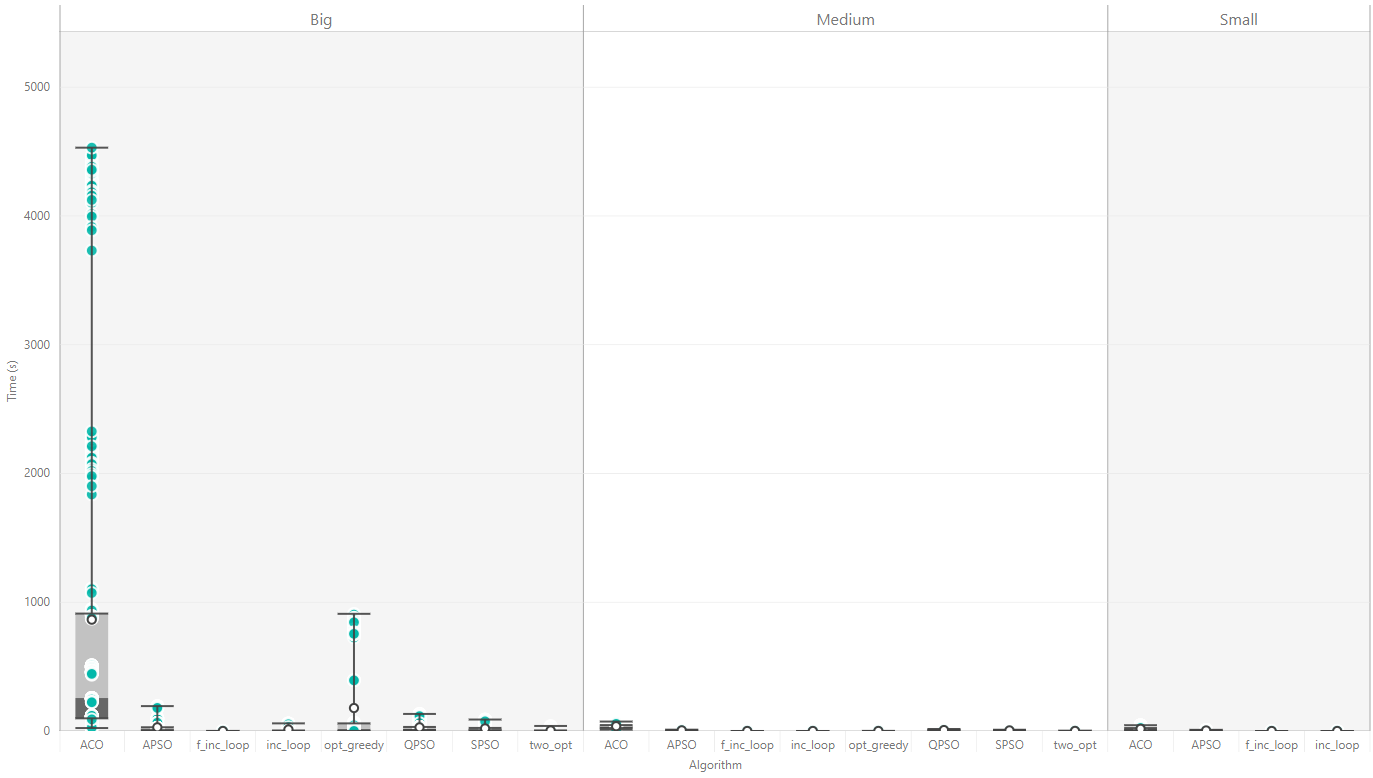
\includegraphics[width=\textwidth]{boxplot_time_nodesize.png}
    		\caption{Computation Time of each algorithm based on the TSP classification}
    		\label{fig:boxPlotTime}
    \end{figure*}
	    
   \begin{center}
        \begin{longtable}[ht]{|l|l|r|r|r|r|r|r|r|}
            \hline  \multicolumn{1}{|c|}{\textbf{TSP}} & 
                    \multicolumn{1}{c|}{\textbf{Algorithm}} & 
                    \multicolumn{1}{c|}{\textbf{Time (s)}} & 
                    \multicolumn{1}{c|}{\textbf{Avg.Dist.}} &
                    \multicolumn{1}{c|}{\textbf{Opt.Dist.}} & 
                    \multicolumn{1}{c|}{\textbf{\%}} &
                    \multicolumn{1}{c|}{\textbf{$\sigma$}} &
                    \multicolumn{1}{c|}{\textbf{MIN}} &
                    \multicolumn{1}{c|}{\textbf{MAX}} \\ \hline 
            \endfirsthead
        
                    \multicolumn{9}{c}%
                    {{\bfseries \tablename\ \thetable{} -- continued from previous page}} \\
                    \hline  \multicolumn{1}{|c|}{\textbf{TSP}} & 
                    \multicolumn{1}{c|}{\textbf{Algorithm}} & 
                    \multicolumn{1}{c|}{\textbf{Time (s)}} & 
                    \multicolumn{1}{c|}{\textbf{Avg.Dist.}} &
                    \multicolumn{1}{c|}{\textbf{Opt.Dist.}} & 
                    \multicolumn{1}{c|}{\textbf{\%}} &
                    \multicolumn{1}{c|}{\textbf{$\sigma$}} &
                    \multicolumn{1}{c|}{\textbf{MIN}} &
                    \multicolumn{1}{c|}{\textbf{MAX}}  \\ \hline
             \endhead
                    
                    \hline \multicolumn{7}{|r|}{{Continued on next page}} \\ \hline
             \endfoot
                    
                    \hline \hline
             \endlastfoot
berlin52 & aco-100 & 2265.04 & 8236.87 & 7542 & 9.21 \% & 184.53 & 7700.07 & 8607.07 \\ \hline
 & aco-50 & 1159.05 & 8339.96 & 7542 & 10.58 \% & 185.09 & 7738.56 & 8797.58 \\ \hline
 & f\_inc\_loop & 0.13 & 8425.37 & 7542 & 11.71 \% & 282.64 & 7694.86 & 9061.57 \\ \hline
 & inc\_loop & 0.14 & 8817.66 & 7542 & 16.91 \% & 194.39 & 8177.8 & 9185.67 \\ \hline
 & opt\_greedy & 4.27 & 8182.19 & 7542 & 8.49 \% & 0 & 8182.19 & 8182.19 \\ \hline
 & pso-apso-100 & 305.17 & 19298.09 & 7542 & 155.87 \% & 0 & 19298.09 & 19298.09 \\ \hline
 & pso-apso-150 & 526.19 & 17755.99 & 7542 & 135.43 \% & 0 & 17755.99 & 17755.99 \\ \hline
 & pso-apso-200 & 667.88 & 18097.81 & 7542 & 139.96 \% & 0 & 18097.81 & 18097.81 \\ \hline
 & pso-apso-50 & 177.5 & 18055.21 & 7542 & 139.4 \% & 0 & 18055.21 & 18055.21 \\ \hline
 & pso-qpso-100 & 457.97 & 18307.2 & 7542 & 142.74 \% & 0 & 18307.2 & 18307.2 \\ \hline
 & pso-qpso-150 & 744.7 & 15647.73 & 7542 & 107.47 \% & 0 & 15647.73 & 15647.73 \\ \hline
 & pso-qpso-200 & 979.59 & 18182.07 & 7542 & 141.08 \% & 0 & 18182.07 & 18182.07 \\ \hline
 & pso-qpso-50 & 242.31 & 22918.04 & 7542 & 203.87 \% & 0 & 22918.04 & 22918.04 \\ \hline
 & pso-spso-100 & 292.28 & 20082.45 & 7542 & 166.27 \% & 0 & 20082.45 & 20082.45 \\ \hline
 & pso-spso-150 & 477.02 & 17357.86 & 7542 & 130.15 \% & 0 & 17357.86 & 17357.86 \\ \hline
 & pso-spso-200 & 595.17 & 21500.51 & 7542 & 185.08 \% & 0 & 21500.51 & 21500.51 \\ \hline
 & pso-spso-50 & 154.89 & 20925.59 & 7542 & 177.45 \% & 0 & 20925.59 & 20925.59 \\ \hline
 & two\_opt & 8.25 & 8352.34 & 7542 & 10.74 \% & 313.98 & 7659.25 & 9281.38 \\ \hline
burma14 & aco-100 & 581.63 & 3324.66 & 3323 & 0.05 \% & 4.6 & 3323 & 3346 \\ \hline
 & aco-50 & 310.18 & 3329.23 & 3323 & 0.19 \% & 9.32 & 3323 & 3359 \\ \hline
 & f\_inc\_loop & 0.03 & 3427.14 & 3323 & 3.13 \% & 90.67 & 3323 & 3734 \\ \hline
 & inc\_loop & 0.03 & 3436.91 & 3323 & 3.43 \% & 73.06 & 3336 & 3684 \\ \hline
 & opt\_greedy & 0.18 & 3841 & 3323 & 15.59 \% & 0 & 3841 & 3841 \\ \hline
 & pso-apso-100 & 258.62 & 3647 & 3323 & 9.75 \% & 0 & 3647 & 3647 \\ \hline
 & pso-apso-150 & 422.94 & 3776 & 3323 & 13.63 \% & 0 & 3776 & 3776 \\ \hline
 & pso-apso-200 & 555.07 & 3839 & 3323 & 15.53 \% & 0 & 3839 & 3839 \\ \hline
 & pso-apso-50 & 132.75 & 3585 & 3323 & 7.88 \% & 0 & 3585 & 3585 \\ \hline
 & pso-qpso-100 & 396.49 & 3693 & 3323 & 11.13 \% & 0 & 3693 & 3693 \\ \hline
 & pso-qpso-150 & 644.15 & 3394 & 3323 & 2.14 \% & 0 & 3394 & 3394 \\ \hline
 & pso-qpso-200 & 837.16 & 3369 & 3323 & 1.38 \% & 0 & 3369 & 3369 \\ \hline
 & pso-qpso-50 & 205.38 & 3446 & 3323 & 3.7 \% & 0 & 3446 & 3446 \\ \hline
 & pso-spso-100 & 255.12 & 3390 & 3323 & 2.02 \% & 0 & 3390 & 3390 \\ \hline
 & pso-spso-150 & 415.52 & 3507 & 3323 & 5.54 \% & 0 & 3507 & 3507 \\ \hline
 & pso-spso-200 & 519.13 & 3836 & 3323 & 15.44 \% & 0 & 3836 & 3836 \\ \hline
 & pso-spso-50 & 131.89 & 3892 & 3323 & 17.12 \% & 0 & 3892 & 3892 \\ \hline
 & two\_opt & 0.35 & 3397.18 & 3323 & 2.23 \% & 72.44 & 3323 & 3565 \\ \hline
ch130 & aco-100 & 5885.39 & 7696.77 & 6110 & 25.97 \% & 173.74 & 7139.54 & 8024.73 \\ \hline
 & aco-50 & 2960.71 & 7873.82 & 6110 & 28.87 \% & 158.56 & 7497.14 & 8269.16 \\ \hline
 & f\_inc\_loop & 0.24 & 6670.1 & 6110 & 9.17 \% & 155.72 & 6362.63 & 7092.71 \\ \hline
 & inc\_loop & 0.97 & 7056.62 & 6110 & 15.49 \% & 167.98 & 6640.12 & 7500.79 \\ \hline
 & opt\_greedy & 26.9 & 7198.74 & 6110 & 17.82 \% & 0 & 7198.74 & 7198.74 \\ \hline
 & pso-apso-100 & 398.63 & 38795.89 & 6110 & 534.96 \% & 0 & 38795.89 & 38795.89 \\ \hline
 & pso-apso-150 & 649.1 & 39045.1 & 6110 & 539.04 \% & 0 & 39045.1 & 39045.1 \\ \hline
 & pso-apso-200 & 858.8 & 39504.72 & 6110 & 546.56 \% & 0 & 39504.72 & 39504.72 \\ \hline
 & pso-apso-50 & 205.47 & 38958.32 & 6110 & 537.62 \% & 0 & 38958.32 & 38958.32 \\ \hline
 & pso-qpso-100 & 591.76 & 39271.63 & 6110 & 542.74 \% & 0 & 39271.63 & 39271.63 \\ \hline
 & pso-qpso-150 & 918.76 & 38471.07 & 6110 & 529.64 \% & 0 & 38471.07 & 38471.07 \\ \hline
 & pso-qpso-200 & 1283.06 & 39057.81 & 6110 & 539.24 \% & 0 & 39057.81 & 39057.81 \\ \hline
 & pso-qpso-50 & 302.79 & 39921.69 & 6110 & 553.38 \% & 0 & 39921.69 & 39921.69 \\ \hline
 & pso-spso-100 & 376.75 & 38539.8 & 6110 & 530.77 \% & 0 & 38539.8 & 38539.8 \\ \hline
 & pso-spso-150 & 595.83 & 37609.83 & 6110 & 515.55 \% & 0 & 37609.83 & 37609.83 \\ \hline
 & pso-spso-200 & 787.42 & 38292.59 & 6110 & 526.72 \% & 0 & 38292.59 & 38292.59 \\ \hline
 & pso-spso-50 & 194.45 & 39125.04 & 6110 & 540.34 \% & 0 & 39125.04 & 39125.04 \\ \hline
 & two\_opt & 89.91 & 7388.01 & 6110 & 20.92 \% & 349.67 & 6879.27 & 8428.68 \\ \hline
ch150 & aco-100 & 6841.79 & 8275.68 & 6528 & 26.77 \% & 175.28 & 7796.37 & 8664.78 \\ \hline
 & aco-50 & 3436.79 & 8432.12 & 6528 & 29.17 \% & 211.82 & 7713.76 & 8857.32 \\ \hline
 & f\_inc\_loop & 0.27 & 7264.3 & 6528 & 11.28 \% & 151.16 & 6906.88 & 7579.71 \\ \hline
 & inc\_loop & 1.2 & 7767.65 & 6528 & 18.99 \% & 150.45 & 7394.53 & 8160.11 \\ \hline
 & opt\_greedy & 25.9 & 7078.44 & 6528 & 8.43 \% & 0 & 7078.44 & 7078.44 \\ \hline
 & pso-apso-100 & 421.71 & 45634.01 & 6528 & 599.05 \% & 0 & 45634.01 & 45634.01 \\ \hline
 & pso-apso-150 & 678.38 & 45206.8 & 6528 & 592.51 \% & 0 & 45206.8 & 45206.8 \\ \hline
 & pso-apso-200 & 885.95 & 45964.54 & 6528 & 604.11 \% & 0 & 45964.54 & 45964.54 \\ \hline
 & pso-apso-50 & 217.6 & 44954.75 & 6528 & 588.65 \% & 0 & 44954.75 & 44954.75 \\ \hline
 & pso-qpso-100 & 620.34 & 46238.99 & 6528 & 608.32 \% & 0 & 46238.99 & 46238.99 \\ \hline
 & pso-qpso-150 & 964.53 & 45138.02 & 6528 & 591.45 \% & 0 & 45138.02 & 45138.02 \\ \hline
 & pso-qpso-200 & 1269.07 & 45875.31 & 6528 & 602.75 \% & 0 & 45875.31 & 45875.31 \\ \hline
 & pso-qpso-50 & 317.47 & 47097.2 & 6528 & 621.46 \% & 0 & 47097.2 & 47097.2 \\ \hline
 & pso-spso-100 & 400.09 & 44083.85 & 6528 & 575.3 \% & 0 & 44083.85 & 44083.85 \\ \hline
 & pso-spso-150 & 625.08 & 45559.98 & 6528 & 597.92 \% & 0 & 45559.98 & 45559.98 \\ \hline
 & pso-spso-200 & 802.1 & 44539.31 & 6528 & 582.28 \% & 0 & 44539.31 & 44539.31 \\ \hline
 & pso-spso-50 & 206.55 & 47443.96 & 6528 & 626.78 \% & 0 & 47443.96 & 47443.96 \\ \hline
 & two\_opt & 153.17 & 8441.34 & 6528 & 29.31 \% & 461.54 & 7609.29 & 9903.75 \\ \hline
eil101 & aco-100 & 4408.35 & 802.7 & 629 & 27.62 \% & 12.07 & 767.9 & 827.1 \\ \hline
 & aco-50 & 2211.07 & 813.76 & 629 & 29.37 \% & 15.82 & 761.12 & 843.16 \\ \hline
 & f\_inc\_loop & 0.17 & 698.67 & 629 & 11.08 \% & 10.93 & 672.02 & 723.06 \\ \hline
 & inc\_loop & 0.47 & 718.18 & 629 & 14.18 \% & 11.39 & 690.33 & 749.92 \\ \hline
 & opt\_greedy & 10.34 & 736.37 & 629 & 17.07 \% & 0 & 736.37 & 736.37 \\ \hline
 & pso-apso-100 & 367.69 & 2438.94 & 629 & 287.75 \% & 0 & 2438.94 & 2438.94 \\ \hline
 & pso-apso-150 & 585.46 & 2504.42 & 629 & 298.16 \% & 0 & 2504.42 & 2504.42 \\ \hline
 & pso-apso-200 & 759.41 & 2563 & 629 & 307.47 \% & 0 & 2563 & 2563 \\ \hline
 & pso-apso-50 & 188.11 & 2539.24 & 629 & 303.69 \% & 0 & 2539.24 & 2539.24 \\ \hline
 & pso-qpso-100 & 541.49 & 2839.98 & 629 & 351.51 \% & 0 & 2839.98 & 2839.98 \\ \hline
 & pso-qpso-150 & 845.33 & 2774.02 & 629 & 341.02 \% & 0 & 2774.02 & 2774.02 \\ \hline
 & pso-qpso-200 & 1097.26 & 2632.6 & 629 & 318.54 \% & 0 & 2632.6 & 2632.6 \\ \hline
 & pso-qpso-50 & 276.47 & 2669.53 & 629 & 324.41 \% & 0 & 2669.53 & 2669.53 \\ \hline
 & pso-spso-100 & 347.16 & 2696.21 & 629 & 328.65 \% & 0 & 2696.21 & 2696.21 \\ \hline
 & pso-spso-150 & 556.1 & 2702.61 & 629 & 329.67 \% & 0 & 2702.61 & 2702.61 \\ \hline
 & pso-spso-200 & 692.92 & 2651.63 & 629 & 321.56 \% & 0 & 2651.63 & 2651.63 \\ \hline
 & pso-spso-50 & 180.17 & 2728.15 & 629 & 333.73 \% & 0 & 2728.15 & 2728.15 \\ \hline
 & two\_opt & 21.99 & 741.55 & 629 & 17.89 \% & 20.61 & 703.57 & 822.05 \\ \hline
eil51 & aco-100 & 2124.31 & 483.95 & 426 & 13.6 \% & 10.27 & 456.95 & 503.17 \\ \hline
 & aco-50 & 1056.01 & 493 & 426 & 15.73 \% & 10.46 & 460.14 & 514.75 \\ \hline
 & f\_inc\_loop & 0.08 & 460.73 & 426 & 8.15 \% & 10.18 & 439.41 & 489.43 \\ \hline
 & inc\_loop & 0.13 & 482.26 & 426 & 13.21 \% & 13.9 & 446.06 & 515.02 \\ \hline
 & opt\_greedy & 2.42 & 505.77 & 426 & 18.73 \% & 0 & 505.77 & 505.77 \\ \hline
 & pso-apso-100 & 308.1 & 973.39 & 426 & 128.5 \% & 0 & 973.39 & 973.39 \\ \hline
 & pso-apso-150 & 495.29 & 959.8 & 426 & 125.31 \% & 0 & 959.8 & 959.8 \\ \hline
 & pso-apso-200 & 630.19 & 945.51 & 426 & 121.95 \% & 0 & 945.51 & 945.51 \\ \hline
 & pso-apso-50 & 155.37 & 1129.03 & 426 & 165.03 \% & 0 & 1129.03 & 1129.03 \\ \hline
 & pso-qpso-100 & 461.57 & 1041.62 & 426 & 144.51 \% & 0 & 1041.62 & 1041.62 \\ \hline
 & pso-qpso-150 & 736.83 & 1195.12 & 426 & 180.54 \% & 0 & 1195.12 & 1195.12 \\ \hline
 & pso-qpso-200 & 941.31 & 1146.84 & 426 & 169.21 \% & 0 & 1146.84 & 1146.84 \\ \hline
 & pso-qpso-50 & 234.9 & 1083.72 & 426 & 154.39 \% & 0 & 1083.72 & 1083.72 \\ \hline
 & pso-spso-100 & 294.32 & 1092.16 & 426 & 156.37 \% & 0 & 1092.16 & 1092.16 \\ \hline
 & pso-spso-150 & 465.3 & 1183.06 & 426 & 177.71 \% & 0 & 1183.06 & 1183.06 \\ \hline
 & pso-spso-200 & 596.36 & 1033.83 & 426 & 142.68 \% & 0 & 1033.83 & 1033.83 \\ \hline
 & pso-spso-50 & 151.1 & 1408.44 & 426 & 230.62 \% & 0 & 1408.44 & 1408.44 \\ \hline
 & two\_opt & 3.16 & 464.66 & 426 & 9.07 \% & 13.13 & 444.48 & 502.73 \\ \hline
eil76 & aco-100 & 3251.41 & 638.04 & 538 & 18.6 \% & 13.01 & 590.11 & 662.27 \\ \hline
 & aco-50 & 1635.36 & 647.74 & 538 & 20.4 \% & 14.24 & 612.15 & 679.72 \\ \hline
 & f\_inc\_loop & 0.15 & 592.18 & 538 & 10.07 \% & 10.11 & 568.63 & 615.62 \\ \hline
 & inc\_loop & 0.26 & 605.07 & 538 & 12.47 \% & 13.12 & 575.05 & 632.54 \\ \hline
 & opt\_greedy & 6.64 & 612.66 & 538 & 13.88 \% & 0 & 612.66 & 612.66 \\ \hline
 & pso-apso-100 & 334.95 & 1806.96 & 538 & 235.87 \% & 0 & 1806.96 & 1806.96 \\ \hline
 & pso-apso-150 & 532 & 1678.56 & 538 & 212 \% & 0 & 1678.56 & 1678.56 \\ \hline
 & pso-apso-200 & 694.19 & 1715.39 & 538 & 218.85 \% & 0 & 1715.39 & 1715.39 \\ \hline
 & pso-apso-50 & 169.35 & 1862.94 & 538 & 246.27 \% & 0 & 1862.94 & 1862.94 \\ \hline
 & pso-qpso-100 & 500.63 & 1969.19 & 538 & 266.02 \% & 0 & 1969.19 & 1969.19 \\ \hline
 & pso-qpso-150 & 806.52 & 1969.55 & 538 & 266.09 \% & 0 & 1969.55 & 1969.55 \\ \hline
 & pso-qpso-200 & 1017.27 & 2016.99 & 538 & 274.91 \% & 0 & 2016.99 & 2016.99 \\ \hline
 & pso-qpso-50 & 251.74 & 1989.73 & 538 & 269.84 \% & 0 & 1989.73 & 1989.73 \\ \hline
 & pso-spso-100 & 324.87 & 1995.52 & 538 & 270.91 \% & 0 & 1995.52 & 1995.52 \\ \hline
 & pso-spso-150 & 511.66 & 1822.66 & 538 & 238.79 \% & 0 & 1822.66 & 1822.66 \\ \hline
 & pso-spso-200 & 653.7 & 1947.61 & 538 & 262.01 \% & 0 & 1947.61 & 1947.61 \\ \hline
 & pso-spso-50 & 162.73 & 2015.59 & 538 & 274.64 \% & 0 & 2015.59 & 2015.59 \\ \hline
 & two\_opt & 12.41 & 614.62 & 538 & 14.24 \% & 17.86 & 574.1 & 662.89 \\ \hline
gr202 & aco-100 & 9641.57 & 52804.79 & 40160 & 31.49 \% & 715.43 & 50758 & 54222 \\ \hline
 & aco-50 & 4812.57 & 53999.84 & 40160 & 34.46 \% & 934.6 & 50852 & 55933 \\ \hline
 & f\_inc\_loop & 0.44 & 43920.47 & 40160 & 9.36 \% & 777.07 & 42104 & 45561 \\ \hline
 & inc\_loop & 2.59 & 46574.78 & 40160 & 15.97 \% & 468.46 & 44624 & 47454 \\ \hline
 & opt\_greedy & 50.88 & 47060 & 40160 & 17.18 \% & 0 & 47060 & 47060 \\ \hline
 & pso-apso-100 & 495.79 & 211214 & 40160 & 425.93 \% & 0 & 211214 & 211214 \\ \hline
 & pso-apso-150 & 792.25 & 197806 & 40160 & 392.54 \% & 0 & 197806 & 197806 \\ \hline
 & pso-apso-200 & 1030.69 & 211880 & 40160 & 427.59 \% & 0 & 211880 & 211880 \\ \hline
 & pso-apso-50 & 255.18 & 206927 & 40160 & 415.26 \% & 0 & 206927 & 206927 \\ \hline
 & pso-qpso-100 & 699.9 & 148348 & 40160 & 269.39 \% & 0 & 148348 & 148348 \\ \hline
 & pso-qpso-150 & 1090.58 & 144666 & 40160 & 260.22 \% & 0 & 144666 & 144666 \\ \hline
 & pso-qpso-200 & 1406.27 & 143832 & 40160 & 258.15 \% & 0 & 143832 & 143832 \\ \hline
 & pso-qpso-50 & 357.53 & 161412 & 40160 & 301.92 \% & 0 & 161412 & 161412 \\ \hline
 & pso-spso-100 & 459.79 & 200944 & 40160 & 400.36 \% & 0 & 200944 & 200944 \\ \hline
 & pso-spso-150 & 717.36 & 193691 & 40160 & 382.3 \% & 0 & 193691 & 193691 \\ \hline
 & pso-spso-200 & 914.54 & 192811 & 40160 & 380.11 \% & 0 & 192811 & 192811 \\ \hline
 & pso-spso-50 & 237.6 & 194242 & 40160 & 383.67 \% & 0 & 194242 & 194242 \\ \hline
 & two\_opt & 77.51 & 49031.62 & 40160 & 22.09 \% & 1943.55 & 45719 & 55583 \\ \hline
gr666 & aco-100 & 48927.56 & 458693.54 & 294358 & 55.83 \% & 7552.12 & 430686 & 469732 \\ \hline
 & aco-50 & 24647.11 & 481753.34 & 294358 & 63.66 \% & 8828.58 & 456603 & 497367 \\ \hline
 & f\_inc\_loop & 4.12 & 334608.28 & 294358 & 13.67 \% & 5031.84 & 320830 & 354021 \\ \hline
 & inc\_loop & 114.27 & 347084.87 & 294358 & 17.91 \% & 4158.42 & 337200 & 360891 \\ \hline
 & opt\_greedy & 1603.41 & 350243 & 294358 & 18.99 \% & 0 & 350243 & 350243 \\ \hline
 & pso-apso-100 & 1300.9 & 4351706 & 294358 & 1378.37 \% & 0 & 4351706 & 4351706 \\ \hline
 & pso-apso-150 & 2028.77 & 4406126 & 294358 & 1396.86 \% & 0 & 4406126 & 4406126 \\ \hline
 & pso-apso-200 & 2738.81 & 4128698 & 294358 & 1302.61 \% & 0 & 4128698 & 4128698 \\ \hline
 & pso-apso-50 & 636.98 & 4491834 & 294358 & 1425.98 \% & 0 & 4491834 & 4491834 \\ \hline
 & pso-qpso-100 & 1509.97 & 3408750 & 294358 & 1058.03 \% & 0 & 3408750 & 3408750 \\ \hline
 & pso-qpso-150 & 2280.39 & 3326477 & 294358 & 1030.08 \% & 0 & 3326477 & 3326477 \\ \hline
 & pso-qpso-200 & 2952.13 & 3408083 & 294358 & 1057.8 \% & 0 & 3408083 & 3408083 \\ \hline
 & pso-qpso-50 & 760.93 & 3573902 & 294358 & 1114.13 \% & 0 & 3573902 & 3573902 \\ \hline
 & pso-spso-100 & 1127.73 & 4084973 & 294358 & 1287.76 \% & 0 & 4084973 & 4084973 \\ \hline
 & pso-spso-150 & 1743.18 & 4046883 & 294358 & 1274.82 \% & 0 & 4046883 & 4046883 \\ \hline
 & pso-spso-200 & 2228.19 & 3901777 & 294358 & 1225.52 \% & 0 & 3901777 & 3901777 \\ \hline
 & pso-spso-50 & 582.58 & 4079040 & 294358 & 1285.74 \% & 0 & 4079040 & 4079040 \\ \hline
 & two\_opt & 841.23 & 419215.5 & 294358 & 42.42 \% & 4071.68 & 406334 & 423710 \\ \hline
gr96 & aco-100 & 4144.42 & 65268.96 & 55209 & 18.22 \% & 1490.16 & 60767 & 67823 \\ \hline
 & aco-50 & 2086.73 & 66004.87 & 55209 & 19.55 \% & 1656.13 & 61945 & 69582 \\ \hline
 & f\_inc\_loop & 0.17 & 59932.82 & 55209 & 8.56 \% & 1653.61 & 56070 & 64670 \\ \hline
 & inc\_loop & 0.39 & 64756.28 & 55209 & 17.29 \% & 2841.87 & 58147 & 70243 \\ \hline
 & opt\_greedy & 9.07 & 63945 & 55209 & 15.82 \% & 0 & 63945 & 63945 \\ \hline
 & pso-apso-100 & 361.38 & 209085 & 55209 & 278.72 \% & 0 & 209085 & 209085 \\ \hline
 & pso-apso-150 & 584.86 & 226759 & 55209 & 310.73 \% & 0 & 226759 & 226759 \\ \hline
 & pso-apso-200 & 750.74 & 182426 & 55209 & 230.43 \% & 0 & 182426 & 182426 \\ \hline
 & pso-apso-50 & 183.05 & 237038 & 55209 & 329.35 \% & 0 & 237038 & 237038 \\ \hline
 & pso-qpso-100 & 526.09 & 164948 & 55209 & 198.77 \% & 0 & 164948 & 164948 \\ \hline
 & pso-qpso-150 & 836.18 & 139518 & 55209 & 152.71 \% & 0 & 139518 & 139518 \\ \hline
 & pso-qpso-200 & 1078.54 & 150974 & 55209 & 173.46 \% & 0 & 150974 & 150974 \\ \hline
 & pso-qpso-50 & 273.17 & 162608 & 55209 & 194.53 \% & 0 & 162608 & 162608 \\ \hline
 & pso-spso-100 & 342.47 & 216591 & 55209 & 292.31 \% & 0 & 216591 & 216591 \\ \hline
 & pso-spso-150 & 550.34 & 168904 & 55209 & 205.94 \% & 0 & 168904 & 168904 \\ \hline
 & pso-spso-200 & 686.35 & 181811 & 55209 & 229.31 \% & 0 & 181811 & 181811 \\ \hline
 & pso-spso-50 & 182.51 & 243547 & 55209 & 341.14 \% & 0 & 243547 & 243547 \\ \hline
 & two\_opt & 5.65 & 63394.18 & 55209 & 14.83 \% & 2668.02 & 58766 & 70052 \\ \hline
kroA100 & aco-100 & 4407.2 & 26100.86 & 21282 & 22.64 \% & 611.85 & 24418.46 & 27162.83 \\ \hline
 & aco-50 & 2239.46 & 26577.57 & 21282 & 24.88 \% & 768.01 & 24613.68 & 28493.24 \\ \hline
 & f\_inc\_loop & 0.65 & 23091.76 & 21282 & 8.5 \% & 720.78 & 21762.51 & 25177.63 \\ \hline
 & inc\_loop & 2.22 & 24488.63 & 21282 & 15.07 \% & 680.05 & 22560.99 & 26521.42 \\ \hline
 & opt\_greedy & 13.78 & 24698.5 & 21282 & 16.05 \% & 0 & 24698.5 & 24698.5 \\ \hline
 & pso-apso-100 & 372.94 & 136097.32 & 21282 & 539.49 \% & 0 & 136097.32 & 136097.32 \\ \hline
 & pso-apso-150 & 599.36 & 136398.7 & 21282 & 540.91 \% & 0 & 136398.7 & 136398.7 \\ \hline
 & pso-apso-200 & 778.13 & 129627.75 & 21282 & 509.1 \% & 0 & 129627.75 & 129627.75 \\ \hline
 & pso-apso-50 & 189.29 & 137190.23 & 21282 & 544.63 \% & 0 & 137190.23 & 137190.23 \\ \hline
 & pso-qpso-100 & 553.05 & 132703.14 & 21282 & 523.55 \% & 0 & 132703.14 & 132703.14 \\ \hline
 & pso-qpso-150 & 864.67 & 131829.65 & 21282 & 519.44 \% & 0 & 131829.65 & 131829.65 \\ \hline
 & pso-qpso-200 & 1103.96 & 134368.68 & 21282 & 531.37 \% & 0 & 134368.68 & 134368.68 \\ \hline
 & pso-qpso-50 & 277.62 & 139160.21 & 21282 & 553.89 \% & 0 & 139160.21 & 139160.21 \\ \hline
 & pso-spso-100 & 354.45 & 134263.78 & 21282 & 530.88 \% & 0 & 134263.78 & 134263.78 \\ \hline
 & pso-spso-150 & 561.76 & 131779.46 & 21282 & 519.21 \% & 0 & 131779.46 & 131779.46 \\ \hline
 & pso-spso-200 & 711.47 & 137308.3 & 21282 & 545.19 \% & 0 & 137308.3 & 137308.3 \\ \hline
 & pso-spso-50 & 178.64 & 135109.1 & 21282 & 534.85 \% & 0 & 135109.1 & 135109.1 \\ \hline
 & two\_opt & 41.3 & 25201.01 & 21282 & 18.41 \% & 1194.06 & 22343.74 & 29121.31 \\ \hline
kroC100 & aco-100 & 4434.21 & 24984.31 & 20749 & 20.41 \% & 684.99 & 22754.14 & 25951.33 \\ \hline
 & aco-50 & 2223 & 25403.7 & 20749 & 22.43 \% & 637.92 & 23547.99 & 27133.87 \\ \hline
 & f\_inc\_loop & 0.19 & 22610.52 & 20749 & 8.97 \% & 545.06 & 21513.14 & 24348.71 \\ \hline
 & inc\_loop & 0.43 & 24422.8 & 20749 & 17.71 \% & 828.53 & 22166.36 & 26078.16 \\ \hline
 & opt\_greedy & 17.42 & 23566.4 & 20749 & 13.58 \% & 0 & 23566.4 & 23566.4 \\ \hline
 & pso-apso-100 & 374.74 & 133001.54 & 20749 & 541 \% & 0 & 133001.54 & 133001.54 \\ \hline
 & pso-apso-150 & 599.83 & 131645.92 & 20749 & 534.47 \% & 0 & 131645.92 & 131645.92 \\ \hline
 & pso-apso-200 & 775.41 & 133489.43 & 20749 & 543.35 \% & 0 & 133489.43 & 133489.43 \\ \hline
 & pso-apso-50 & 188.68 & 136689.97 & 20749 & 558.78 \% & 0 & 136689.97 & 136689.97 \\ \hline
 & pso-qpso-100 & 550.94 & 130673.46 & 20749 & 529.78 \% & 0 & 130673.46 & 130673.46 \\ \hline
 & pso-qpso-150 & 863.69 & 134922.05 & 20749 & 550.26 \% & 0 & 134922.05 & 134922.05 \\ \hline
 & pso-qpso-200 & 1097.33 & 131269.53 & 20749 & 532.65 \% & 0 & 131269.53 & 131269.53 \\ \hline
 & pso-qpso-50 & 279.65 & 135164.95 & 20749 & 551.43 \% & 0 & 135164.95 & 135164.95 \\ \hline
 & pso-spso-100 & 350.78 & 130080.84 & 20749 & 526.93 \% & 0 & 130080.84 & 130080.84 \\ \hline
 & pso-spso-150 & 571.93 & 129039.17 & 20749 & 521.91 \% & 0 & 129039.17 & 129039.17 \\ \hline
 & pso-spso-200 & 709.37 & 124951.8 & 20749 & 502.21 \% & 0 & 124951.8 & 124951.8 \\ \hline
 & pso-spso-50 & 182.69 & 133891.02 & 20749 & 545.29 \% & 0 & 133891.02 & 133891.02 \\ \hline
 & two\_opt & 33.3 & 24849.14 & 20749 & 19.76 \% & 1413.94 & 22629 & 29718.89 \\ \hline
kroD100 & aco-100 & 4451.49 & 25641.03 & 21294 & 20.41 \% & 476.75 & 23999.45 & 26631.65 \\ \hline
 & aco-50 & 2240.22 & 26022.22 & 21294 & 22.2 \% & 599.74 & 24338.08 & 27116.16 \\ \hline
 & f\_inc\_loop & 0.18 & 23175.24 & 21294 & 8.83 \% & 573.39 & 21841.78 & 24401.49 \\ \hline
 & inc\_loop & 0.46 & 24710.22 & 21294 & 16.04 \% & 701.77 & 23114.38 & 26320.06 \\ \hline
 & opt\_greedy & 10.84 & 24855.8 & 21294 & 16.73 \% & 0 & 24855.8 & 24855.8 \\ \hline
 & pso-apso-100 & 371.94 & 127502.35 & 21294 & 498.77 \% & 0 & 127502.35 & 127502.35 \\ \hline
 & pso-apso-150 & 611.6 & 125672.57 & 21294 & 490.18 \% & 0 & 125672.57 & 125672.57 \\ \hline
 & pso-apso-200 & 768.38 & 130238 & 21294 & 511.62 \% & 0 & 130238 & 130238 \\ \hline
 & pso-apso-50 & 190.9 & 133933.6 & 21294 & 528.97 \% & 0 & 133933.6 & 133933.6 \\ \hline
 & pso-qpso-100 & 547.1 & 131597.48 & 21294 & 518 \% & 0 & 131597.48 & 131597.48 \\ \hline
 & pso-qpso-150 & 865.49 & 128980.2 & 21294 & 505.71 \% & 0 & 128980.2 & 128980.2 \\ \hline
 & pso-qpso-200 & 1111.38 & 129555.11 & 21294 & 508.41 \% & 0 & 129555.11 & 129555.11 \\ \hline
 & pso-qpso-50 & 274.26 & 134102.64 & 21294 & 529.77 \% & 0 & 134102.64 & 134102.64 \\ \hline
 & pso-spso-100 & 350.95 & 125075.13 & 21294 & 487.37 \% & 0 & 125075.13 & 125075.13 \\ \hline
 & pso-spso-150 & 568.05 & 126403.57 & 21294 & 493.61 \% & 0 & 126403.57 & 126403.57 \\ \hline
 & pso-spso-200 & 717.92 & 129221.76 & 21294 & 506.85 \% & 0 & 129221.76 & 129221.76 \\ \hline
 & pso-spso-50 & 184.94 & 121535.63 & 21294 & 470.75 \% & 0 & 121535.63 & 121535.63 \\ \hline
 & two\_opt & 32.88 & 24924.59 & 21294 & 17.05 \% & 1041.19 & 23129.67 & 28389.74 \\ \hline
lin105 & aco-100 & 4657.74 & 16749.66 & 14379 & 16.49 \% & 419.39 & 15596.34 & 17633.8 \\ \hline
 & aco-50 & 2360.69 & 17060.06 & 14379 & 18.65 \% & 477.18 & 15640.59 & 18206.24 \\ \hline
 & f\_inc\_loop & 0.18 & 15860.13 & 14379 & 10.3 \% & 396.47 & 14840.72 & 17018.1 \\ \hline
 & inc\_loop & 0.51 & 17022.58 & 14379 & 18.39 \% & 560.86 & 15828.34 & 18201.03 \\ \hline
 & opt\_greedy & 11.56 & 16939.44 & 14379 & 17.81 \% & 0 & 16939.44 & 16939.44 \\ \hline
 & pso-apso-100 & 379.52 & 80167.92 & 14379 & 457.53 \% & 0 & 80167.92 & 80167.92 \\ \hline
 & pso-apso-150 & 617.98 & 71804.99 & 14379 & 399.37 \% & 0 & 71804.99 & 71804.99 \\ \hline
 & pso-apso-200 & 784.18 & 68635.69 & 14379 & 377.33 \% & 0 & 68635.69 & 68635.69 \\ \hline
 & pso-apso-50 & 193.53 & 74089.44 & 14379 & 415.26 \% & 0 & 74089.44 & 74089.44 \\ \hline
 & pso-qpso-100 & 553.75 & 56150.42 & 14379 & 290.5 \% & 0 & 56150.42 & 56150.42 \\ \hline
 & pso-qpso-150 & 873.59 & 48541.49 & 14379 & 237.59 \% & 0 & 48541.49 & 48541.49 \\ \hline
 & pso-qpso-200 & 1116.07 & 46208.14 & 14379 & 221.36 \% & 0 & 46208.14 & 46208.14 \\ \hline
 & pso-qpso-50 & 282.37 & 53148.22 & 14379 & 269.62 \% & 0 & 53148.22 & 53148.22 \\ \hline
 & pso-spso-100 & 360.95 & 66070.67 & 14379 & 359.49 \% & 0 & 66070.67 & 66070.67 \\ \hline
 & pso-spso-150 & 577.7 & 63343.04 & 14379 & 340.52 \% & 0 & 63343.04 & 63343.04 \\ \hline
 & pso-spso-200 & 719.67 & 57616.65 & 14379 & 300.7 \% & 0 & 57616.65 & 57616.65 \\ \hline
 & pso-spso-50 & 184.95 & 65117.8 & 14379 & 352.87 \% & 0 & 65117.8 & 65117.8 \\ \hline
 & two\_opt & 18.8 & 17240.81 & 14379 & 19.9 \% & 840.76 & 15557.94 & 20008.42 \\ \hline
pr1002 & aco-100 & 89526.28 & 453823.16 & 259045 & 75.19 \% & 6034.46 & 432512.18 & 463697.73 \\ \hline
 & aco-50 & 44797.11 & 482237.11 & 259045 & 86.16 \% & 7478.98 & 453680.83 & 495023.6 \\ \hline
 & f\_inc\_loop & 8.56 & 292135.23 & 259045 & 12.77 \% & 2558.52 & 285620.02 & 298310.16 \\ \hline
 & inc\_loop & 388.55 & 301216.88 & 259045 & 16.28 \% & 2574.58 & 293699.67 & 309751.06 \\ \hline
 & opt\_greedy & 5525.38 & 312237.27 & 259045 & 20.53 \% & 0 & 312237.27 & 312237.27 \\ \hline
 & pso-apso-100 & 1987.77 & 5586377.93 & 259045 & 2056.53 \% & 0 & 5586377.93 & 5586377.93 \\ \hline
 & pso-apso-150 & 3022.24 & 5746239.95 & 259045 & 2118.24 \% & 0 & 5746239.95 & 5746239.95 \\ \hline
 & pso-apso-200 & 4078.99 & 5489574.44 & 259045 & 2019.16 \% & 0.11 & 5489574.44 & 5489574.44 \\ \hline
 & pso-apso-50 & 1020.95 & 5700604.23 & 259045 & 2100.62 \% & 0 & 5700604.23 & 5700604.23 \\ \hline
 & pso-qpso-100 & 2138.59 & 4654134.94 & 259045 & 1696.65 \% & 0 & 4654134.94 & 4654134.94 \\ \hline
 & pso-qpso-150 & 3153.35 & 4445011.54 & 259045 & 1615.92 \% & 0 & 4445011.54 & 4445011.54 \\ \hline
 & pso-qpso-200 & 4179.51 & 4381837.86 & 259045 & 1591.54 \% & 0 & 4381837.86 & 4381837.86 \\ \hline
 & pso-qpso-50 & 1083.76 & 4808843.31 & 259045 & 1756.37 \% & 0 & 4808843.31 & 4808843.31 \\ \hline
 & pso-spso-100 & 1773.51 & 5204886.62 & 259045 & 1909.26 \% & 0 & 5204886.62 & 5204886.62 \\ \hline
 & pso-spso-150 & 2534 & 4969495.03 & 259045 & 1818.39 \% & 0 & 4969495.03 & 4969495.03 \\ \hline
 & pso-spso-200 & 3326.83 & 5089123.89 & 259045 & 1864.57 \% & 0.06 & 5089123.89 & 5089123.89 \\ \hline
 & pso-spso-50 & 852.6 & 5304721.91 & 259045 & 1947.8 \% & 0.06 & 5304721.91 & 5304721.91 \\ \hline
 & two\_opt & 926.25 & 348246.58 & 259045 & 34.43 \% & 2346.38 & 333308.81 & 349438.24 \\ \hline
pr2392 & aco-100 & 414119.86 & 758803.69 & 378032 & 100.72 \% & 9151.06 & 735453.04 & 777169.14 \\ \hline
 & aco-50 & 211499.52 & 828058.08 & 378032 & 119.04 \% & 10575.98 & 791295.71 & 845482.94 \\ \hline
 & f\_inc\_loop & 47.55 & 437608.45 & 378032 & 15.76 \% & 2804.39 & 430651.73 & 444002.51 \\ \hline
 & inc\_loop & 5416.46 & 455999.14 & 378032 & 20.62 \% & 2151.88 & 451372.65 & 460240.09 \\ \hline
 & opt\_greedy & 81904.36 & 458789.65 & 378032 & 21.36 \% & 0 & 458789.65 & 458789.65 \\ \hline
 & pso-apso-100 & 4868.08 & 13887665.42 & 378032 & 3573.67 \% & 0 & 13887665.42 & 13887665.42 \\ \hline
 & pso-apso-150 & 9406.84 & 13529590.85 & 378032 & 3478.95 \% & 0 & 13529590.85 & 13529590.85 \\ \hline
 & pso-apso-200 & 18280.38 & 13621714.24 & 378032 & 3503.32 \% & 0.18 & 13621714.24 & 13621714.24 \\ \hline
 & pso-apso-50 & 2336.25 & 13655832.79 & 378032 & 3512.35 \% & 0 & 13655832.79 & 13655832.79 \\ \hline
 & pso-qpso-100 & 6082.04 & 12739768.37 & 378032 & 3270.02 \% & 0 & 12739768.37 & 12739768.37 \\ \hline
 & pso-qpso-150 & 9554.1 & 12585053.92 & 378032 & 3229.1 \% & 0 & 12585053.92 & 12585053.92 \\ \hline
 & pso-qpso-200 & 12217.4 & 12023185.53 & 378032 & 3080.47 \% & 0.18 & 12023185.53 & 12023185.53 \\ \hline
 & pso-qpso-50 & 3046.98 & 12769142.91 & 378032 & 3277.79 \% & 0.18 & 12769142.91 & 12769142.91 \\ \hline
 & pso-spso-100 & 4154.98 & 13204005.65 & 378032 & 3392.83 \% & 0 & 13204005.65 & 13204005.65 \\ \hline
 & pso-spso-150 & 6269.83 & 13126757.49 & 378032 & 3372.39 \% & 0 & 13126757.49 & 13126757.49 \\ \hline
 & pso-spso-200 & 8176.07 & 13098856.98 & 378032 & 3365.01 \% & 0.18 & 13098856.98 & 13098856.98 \\ \hline
 & pso-spso-50 & 2105.91 & 13605994.73 & 378032 & 3499.16 \% & 0 & 13605994.73 & 13605994.73 \\ \hline
 & two\_opt & 22.61 & 378062.83 & 378032 & 0.01 \% & 0 & 378062.83 & 378062.83 \\ \hline
pr76 & aco-100 & 3279.6 & 122719.12 & 108159 & 13.46 \% & 2202.63 & 117488.89 & 127056.17 \\ \hline
 & aco-50 & 1655.52 & 124151.94 & 108159 & 14.79 \% & 2321.81 & 117472.06 & 129675.58 \\ \hline
 & f\_inc\_loop & 0.13 & 116023.25 & 108159 & 7.27 \% & 3190.49 & 109616.78 & 124466.13 \\ \hline
 & inc\_loop & 0.28 & 122439.77 & 108159 & 13.2 \% & 3729.23 & 114185.6 & 130647.45 \\ \hline
 & opt\_greedy & 5.75 & 130921 & 108159 & 21.04 \% & 0 & 130921 & 130921 \\ \hline
 & pso-apso-100 & 341.23 & 314295.21 & 108159 & 190.59 \% & 0 & 314295.21 & 314295.21 \\ \hline
 & pso-apso-150 & 549.17 & 359030.08 & 108159 & 231.95 \% & 0 & 359030.08 & 359030.08 \\ \hline
 & pso-apso-200 & 699.96 & 327419.29 & 108159 & 202.72 \% & 0 & 327419.29 & 327419.29 \\ \hline
 & pso-apso-50 & 171.06 & 346302.83 & 108159 & 220.18 \% & 0 & 346302.83 & 346302.83 \\ \hline
 & pso-qpso-100 & 501.45 & 272633.24 & 108159 & 152.07 \% & 0 & 272633.24 & 272633.24 \\ \hline
 & pso-qpso-150 & 795.2 & 245483.68 & 108159 & 126.97 \% & 0 & 245483.68 & 245483.68 \\ \hline
 & pso-qpso-200 & 1026.5 & 227953.32 & 108159 & 110.76 \% & 0 & 227953.32 & 227953.32 \\ \hline
 & pso-qpso-50 & 257.89 & 290853.6 & 108159 & 168.91 \% & 0 & 290853.6 & 290853.6 \\ \hline
 & pso-spso-100 & 325.39 & 358624.29 & 108159 & 231.57 \% & 0 & 358624.29 & 358624.29 \\ \hline
 & pso-spso-150 & 520.93 & 316286.84 & 108159 & 192.43 \% & 0 & 316286.84 & 316286.84 \\ \hline
 & pso-spso-200 & 643.01 & 275485.24 & 108159 & 154.7 \% & 0 & 275485.24 & 275485.24 \\ \hline
 & pso-spso-50 & 163.27 & 385109.1 & 108159 & 256.06 \% & 0 & 385109.1 & 385109.1 \\ \hline
 & two\_opt & 3.27 & 129474.35 & 108159 & 19.71 \% & 6315.25 & 111934.95 & 145197.34 \\ \hline
rd100 & aco-100 & 4413.83 & 9891.62 & 7910 & 25.05 \% & 220.06 & 9143.86 & 10303.68 \\ \hline
 & aco-50 & 2214.92 & 10057.32 & 7910 & 27.15 \% & 249.66 & 9304.74 & 10568.33 \\ \hline
 & f\_inc\_loop & 0.17 & 8678.43 & 7910 & 9.71 \% & 251.46 & 8002.19 & 9277.06 \\ \hline
 & inc\_loop & 0.44 & 9086.85 & 7910 & 14.88 \% & 213.52 & 8644.89 & 9587.05 \\ \hline
 & opt\_greedy & 10.47 & 9427.33 & 7910 & 19.18 \% & 0 & 9427.33 & 9427.33 \\ \hline
 & pso-apso-100 & 376.81 & 44275.44 & 7910 & 459.74 \% & 0 & 44275.44 & 44275.44 \\ \hline
 & pso-apso-150 & 614.56 & 44794.28 & 7910 & 466.3 \% & 0 & 44794.28 & 44794.28 \\ \hline
 & pso-apso-200 & 782.81 & 44151.65 & 7910 & 458.18 \% & 0 & 44151.65 & 44151.65 \\ \hline
 & pso-apso-50 & 192.2 & 41808.23 & 7910 & 428.55 \% & 0 & 41808.23 & 41808.23 \\ \hline
 & pso-qpso-100 & 551.61 & 45436 & 7910 & 474.41 \% & 0 & 45436 & 45436 \\ \hline
 & pso-qpso-150 & 864.81 & 45073.22 & 7910 & 469.83 \% & 0 & 45073.22 & 45073.22 \\ \hline
 & pso-qpso-200 & 1105.84 & 44698.95 & 7910 & 465.09 \% & 0 & 44698.95 & 44698.95 \\ \hline
 & pso-qpso-50 & 277.09 & 45519.16 & 7910 & 475.46 \% & 0 & 45519.16 & 45519.16 \\ \hline
 & pso-spso-100 & 349.83 & 43824.5 & 7910 & 454.04 \% & 0 & 43824.5 & 43824.5 \\ \hline
 & pso-spso-150 & 575.41 & 43306.23 & 7910 & 447.49 \% & 0 & 43306.23 & 43306.23 \\ \hline
 & pso-spso-200 & 702.75 & 45103.01 & 7910 & 470.2 \% & 0 & 45103.01 & 45103.01 \\ \hline
 & pso-spso-50 & 179.39 & 45100.51 & 7910 & 470.17 \% & 0 & 45100.51 & 45100.51 \\ \hline
 & two\_opt & 30.05 & 9440.72 & 7910 & 19.35 \% & 364.27 & 8673.3 & 10555.51 \\ \hline
st70 & aco-100 & 3025.84 & 797.13 & 675 & 18.09 \% & 16.15 & 758.22 & 824.25 \\ \hline
 & aco-50 & 1508.22 & 808.84 & 675 & 19.83 \% & 18.69 & 763.21 & 846.03 \\ \hline
 & f\_inc\_loop & 0.11 & 724.52 & 675 & 7.34 \% & 17.78 & 694.17 & 771.82 \\ \hline
 & inc\_loop & 0.22 & 755.21 & 675 & 11.88 \% & 23.75 & 709.41 & 808.62 \\ \hline
 & opt\_greedy & 4.53 & 761.69 & 675 & 12.84 \% & 0 & 761.69 & 761.69 \\ \hline
 & pso-apso-100 & 330.51 & 2480.57 & 675 & 267.49 \% & 0 & 2480.57 & 2480.57 \\ \hline
 & pso-apso-150 & 544.94 & 2648.7 & 675 & 292.4 \% & 0 & 2648.7 & 2648.7 \\ \hline
 & pso-apso-200 & 681.68 & 2477.52 & 675 & 267.04 \% & 0 & 2477.52 & 2477.52 \\ \hline
 & pso-apso-50 & 166.9 & 2777.89 & 675 & 311.54 \% & 0 & 2777.89 & 2777.89 \\ \hline
 & pso-qpso-100 & 493.05 & 2879.27 & 675 & 326.56 \% & 0 & 2879.27 & 2879.27 \\ \hline
 & pso-qpso-150 & 789.01 & 2879.97 & 675 & 326.66 \% & 0 & 2879.97 & 2879.97 \\ \hline
 & pso-qpso-200 & 997.68 & 2910.58 & 675 & 331.2 \% & 0 & 2910.58 & 2910.58 \\ \hline
 & pso-qpso-50 & 249.33 & 2606.64 & 675 & 286.17 \% & 0 & 2606.64 & 2606.64 \\ \hline
 & pso-spso-100 & 315.58 & 2588.4 & 675 & 283.47 \% & 0 & 2588.4 & 2588.4 \\ \hline
 & pso-spso-150 & 479.46 & 2634.6 & 675 & 290.31 \% & 0 & 2634.6 & 2634.6 \\ \hline
 & pso-spso-200 & 640.64 & 2906.11 & 675 & 330.54 \% & 0 & 2906.11 & 2906.11 \\ \hline
 & pso-spso-50 & 159.09 & 2934.59 & 675 & 334.75 \% & 0 & 2934.59 & 2934.59 \\ \hline
 & two\_opt & 8.85 & 756.17 & 675 & 12.02 \% & 25.71 & 701.2 & 858.12 \\ \hline
tsp225 & aco-100 & 11119.3 & 5515.97 & 3916 & 40.86 \% & 117.03 & 5016.72 & 5697.63 \\ \hline
 & aco-50 & 5598.57 & 5705.96 & 3916 & 45.71 \% & 123.55 & 5382.33 & 5911.7 \\ \hline
 & f\_inc\_loop & 0.53 & 4318.92 & 3916 & 10.29 \% & 76.34 & 4125.54 & 4485.59 \\ \hline
 & inc\_loop & 3.39 & 4465.02 & 3916 & 14.02 \% & 69.36 & 4261.54 & 4618.41 \\ \hline
 & opt\_greedy & 75.03 & 4633.2 & 3916 & 18.31 \% & 0 & 4633.2 & 4633.2 \\ \hline
 & pso-apso-100 & 542.21 & 32319.5 & 3916 & 725.32 \% & 0 & 32319.5 & 32319.5 \\ \hline
 & pso-apso-150 & 817.46 & 32476.42 & 3916 & 729.33 \% & 0 & 32476.42 & 32476.42 \\ \hline
 & pso-apso-200 & 1097.01 & 32595.68 & 3916 & 732.37 \% & 0 & 32595.68 & 32595.68 \\ \hline
 & pso-apso-50 & 278.4 & 33263.68 & 3916 & 749.43 \% & 0 & 33263.68 & 33263.68 \\ \hline
 & pso-qpso-100 & 754.71 & 24450.75 & 3916 & 524.38 \% & 0 & 24450.75 & 24450.75 \\ \hline
 & pso-qpso-150 & 1126.55 & 25324.44 & 3916 & 546.69 \% & 0 & 25324.44 & 25324.44 \\ \hline
 & pso-qpso-200 & 1503.28 & 23371.2 & 3916 & 496.81 \% & 0 & 23371.2 & 23371.2 \\ \hline
 & pso-qpso-50 & 382.82 & 25277.65 & 3916 & 545.5 \% & 0 & 25277.65 & 25277.65 \\ \hline
 & pso-spso-100 & 505.77 & 30930.42 & 3916 & 689.85 \% & 0 & 30930.42 & 30930.42 \\ \hline
 & pso-spso-150 & 743.16 & 28516.88 & 3916 & 628.21 \% & 0 & 28516.88 & 28516.88 \\ \hline
 & pso-spso-200 & 971.32 & 28788.59 & 3916 & 635.15 \% & 0 & 28788.59 & 28788.59 \\ \hline
 & pso-spso-50 & 257.34 & 31676.63 & 3916 & 708.9 \% & 0 & 31676.63 & 31676.63 \\ \hline
 & two\_opt & 316.7 & 5185.16 & 3916 & 32.41 \% & 291.15 & 4618.5 & 6149.86 \\ \hline
ulysses16 & aco-100 & 666.27 & 6860.24 & 6859 & 0.02 \% & 3.85 & 6859 & 6878 \\ \hline
 & aco-50 & 343.27 & 6870.7 & 6859 & 0.17 \% & 18.26 & 6859 & 6913 \\ \hline
 & f\_inc\_loop & 0.03 & 7081.87 & 6859 & 3.25 \% & 170.32 & 6859 & 7562 \\ \hline
 & inc\_loop & 0.04 & 7320.39 & 6859 & 6.73 \% & 167.63 & 6909 & 7550 \\ \hline
 & opt\_greedy & 0.21 & 7943 & 6859 & 15.8 \% & 0 & 7943 & 7943 \\ \hline
 & pso-apso-100 & 267.36 & 7358 & 6859 & 7.28 \% & 0 & 7358 & 7358 \\ \hline
 & pso-apso-150 & 412.45 & 6952 & 6859 & 1.36 \% & 0 & 6952 & 6952 \\ \hline
 & pso-apso-200 & 539.71 & 7428 & 6859 & 8.3 \% & 0 & 7428 & 7428 \\ \hline
 & pso-apso-50 & 134.32 & 7381 & 6859 & 7.61 \% & 0 & 7381 & 7381 \\ \hline
 & pso-qpso-100 & 404.97 & 7285 & 6859 & 6.21 \% & 0 & 7285 & 7285 \\ \hline
 & pso-qpso-150 & 629.87 & 6950 & 6859 & 1.33 \% & 0 & 6950 & 6950 \\ \hline
 & pso-qpso-200 & 841.98 & 7138 & 6859 & 4.07 \% & 0 & 7138 & 7138 \\ \hline
 & pso-qpso-50 & 203.9 & 7667 & 6859 & 11.78 \% & 0 & 7667 & 7667 \\ \hline
 & pso-spso-100 & 260.41 & 7289 & 6859 & 6.27 \% & 0 & 7289 & 7289 \\ \hline
 & pso-spso-150 & 395.96 & 7469 & 6859 & 8.89 \% & 0 & 7469 & 7469 \\ \hline
 & pso-spso-200 & 523.81 & 7256 & 6859 & 5.79 \% & 0 & 7256 & 7256 \\ \hline
 & pso-spso-50 & 131.64 & 8307 & 6859 & 21.11 \% & 0 & 8307 & 8307 \\ \hline
 & two\_opt & 0.41 & 6962.99 & 6859 & 1.52 \% & 99.51 & 6859 & 7196 \\ \hline
ulysses22 & aco-100 & 922.24 & 7066.48 & 7013 & 0.76 \% & 34.32 & 7013 & 7127 \\ \hline
 & aco-50 & 471.15 & 7088.49 & 7013 & 1.08 \% & 42.12 & 7013 & 7213 \\ \hline
 & f\_inc\_loop & 0.04 & 7312.48 & 7013 & 4.27 \% & 178.35 & 7013 & 7714 \\ \hline
 & inc\_loop & 0.05 & 7613.18 & 7013 & 8.56 \% & 162.75 & 7128 & 8121 \\ \hline
 & opt\_greedy & 0.39 & 8180 & 7013 & 16.64 \% & 0 & 8180 & 8180 \\ \hline
 & pso-apso-100 & 279.78 & 9599 & 7013 & 36.87 \% & 0 & 9599 & 9599 \\ \hline
 & pso-apso-150 & 421.93 & 9074 & 7013 & 29.39 \% & 0 & 9074 & 9074 \\ \hline
 & pso-apso-200 & 554.91 & 9605 & 7013 & 36.96 \% & 0 & 9605 & 9605 \\ \hline
 & pso-apso-50 & 140.89 & 9580 & 7013 & 36.6 \% & 0 & 9580 & 9580 \\ \hline
 & pso-qpso-100 & 422.07 & 8562 & 7013 & 22.09 \% & 0 & 8562 & 8562 \\ \hline
 & pso-qpso-150 & 643.18 & 9137 & 7013 & 30.29 \% & 0 & 9137 & 9137 \\ \hline
 & pso-qpso-200 & 852.69 & 9319 & 7013 & 32.88 \% & 0 & 9319 & 9319 \\ \hline
 & pso-qpso-50 & 212.05 & 8261 & 7013 & 17.8 \% & 0 & 8261 & 8261 \\ \hline
 & pso-spso-100 & 270.91 & 9480 & 7013 & 35.18 \% & 0 & 9480 & 9480 \\ \hline
 & pso-spso-150 & 405.16 & 8447 & 7013 & 20.45 \% & 0 & 8447 & 8447 \\ \hline
 & pso-spso-200 & 537.29 & 8454 & 7013 & 20.55 \% & 0 & 8454 & 8454 \\ \hline
 & pso-spso-50 & 135.97 & 9125 & 7013 & 30.12 \% & 0 & 9125 & 9125 \\ \hline
 & two\_opt & 0.59 & 7176.22 & 7013 & 2.33 \% & 102.41 & 7013 & 7441 \\ \hline
        \caption{Performance Summary} \label{tab:performancesummary} \\	
        \end{longtable}
    \end{center}
\clearpage
\end{document}
